\documentclass[12pt]{report}
\usepackage{geometry}
\usepackage{graphicx}
\usepackage{array}
\usepackage{rotating}
\usepackage{pdflscape}
\usepackage{amsmath}
\usepackage{listings}
\numberwithin{figure}{section}
\numberwithin{table}{section}
\usepackage{float}
\usepackage{gensymb}
\usepackage{fixltx2e}
\usepackage[utf8x]{inputenc}
\usepackage[toc,page]{appendix}
\usepackage{algorithmic}
\usepackage{algorithm}
%border spacing
\geometry{
 a4paper,
 lmargin = 37mm,
 rmargin = 1in,
 tmargin = 1in,
 bmargin = 1in 
 }
 
%line spacing
\renewcommand{\baselinestretch}{1.5}  

\title{An efficient query platform for streaming and dynamic natural graphs}
\author{Milindu Sanoj Kumarage}	

\begin{document} 

\begin{titlepage}
\newgeometry{left=25mm}
\newcommand{\HRule}{\rule{\linewidth}{0.5mm}} % Defines a new command for the horizontal lines, change thickness here
\begin{figure}[H]
\centering

\includegraphics[height=2cm]{uoc}\\[1cm]
\end{figure}
\center 
{ \LARGE \bfseries An efficient query platform for streaming and dynamic natural graphs }\\[1.5cm]
\Large Milindu Sanoj Kumarage\\
\Large Index No: 12000752\\[1cm]
\Large Supervisor: Dr.D.N. Ranasinghe\\[1cm]
\Large December 2016\\[1.5cm]
\large Submitted in partial fulfillment of the requirements of the B. Sc in Computer Science 4th year individual project\\[0.5cm] 

\includegraphics[scale=0.06]{ucsc}
\vfill % Fill the rest of the page with whitespace
\end{titlepage}

\pagenumbering{roman}
\section*{Declaration}
\addcontentsline{toc}{section}{Declaration}%

I certify that this dissertation does not incorporate, without acknowledgement, any material previously submitted for a degree or diploma in any university and to the best of my knowledge and belief, it does not contain any material previously published or written by another person or myself except where due reference is made in the text. I also hereby give consent for my dissertation, if accepted, be made available for photocopying and for interlibrary loans, and for the title and abstract to be made available to outside organizations.



I, Dr. D.N. Ranasinghe, certify that I supervised this thesis entitled ”An efficient query platform for streaming and dynamic natural graphs” is conducted by M.S.Kumar I recommend this thesis to the University of Colombo School of Computing in partial fulfilment of the requirement of the degree of Bachelor of Science (Computer Science).

\newpage

\section*{Acknowledgements}
\addcontentsline{toc}{section}{Acknowledgements}%
To my parents
\newpage


\section*{Abstract}
\addcontentsline{toc}{section}{Abstract}%

Systems these days generate data in massive scale and processing these data to extract useful information has now become a very common practice. With the hype of Big Data, we see Big Graph is also becoming trendy where relationship between in these massive scale data are used to build massive scale graphs and then analysed for more insightful information.

On the other hand, stream processing gaining lot of attention as they provides a way of extracting information in real-time. In most of the scenarios, even an approximated results are good enough if they can be generated in real-time.

This research evaluates the currently available graph analysing frameworks and identifies their strengths and weaknesses. Then proposes a query platform model for streaming graphs by researching and evaluating techniques and approaches which can be used for building such query platform. 

We identified graph summarization as a good technique for such a query platform and discovered TCM sketching as a graph summarizasion model which fits our needs. Then we implemented our model using TCM sketching and evaluated the model with different metrics like Average Relative Error, Number of Effective Queries, Effectiveness of Effective Queries, Confusion Matrix of queries on streaming graphs. Then we evaluate the same with dynamically changing graphs and natural graphs which follows power-low degree distribution. We introduce optimisations which makes the operations of the query platform efficient.

Then the research propose extensions to the TCM model for automatic sketch creation while the graph is building and evaluate the success when using different sketch creation policies. Then we evaluate the contribution of different queries on the accuracy of the automatic sketch creation. Finally we discuss the memory usage and efficiency of the model. 

\textbf{Keywords:} Streaming, graph,  

\newpage

\listoffigures

\listoftables

\tableofcontents

\newpage
\pagenumbering{arabic}



\chapter{Introduction}

\section{Preamble}

Massive scale datasets are getting common in day-to-day business with the expansion of the internet. More and more devices getting connected, more and more services coming online, more and more data generated and at the same time, the need to work on these data is getting more and more prominent.

\paragraph{}

However, modern day datasets no longer fit into one computing node as the amount of collected data are enormously huge.  We need some kind of a grid with thousands of computing nodes which can work on the dataset parallely, which might be distributed even across many geographical areas but connected through a network, communicating and coordinate their actions.

\paragraph{}

In the other hand, mapping these data into graphs and using graph algorithms to query useful information out of these graphs is also a growing need. Business intelligence systems, anomaly detections systems and many more real world use cases with huge financial values exists which needs insights that could be extracted from the relationships in the graphs, which is not easy to extract from traditional databases. We know the story of Google, how it became the search giant with their PageRank\cite{PageRank} algorithm which makes use of graph relations to rank the web pages of the World Wide Web and to produce the users the most related web pages to their queries. In the same way, Facebook uses their social graph with trillion edges\cite{Facebook} to uncover new insights about their users, products, and interactions.

\paragraph{}

With the popularity of the use cases like above, the need of betters platforms which can perform graph computations efficiently in parallel on largely distributed clusters aroused. Query platforms makes it easier to query for data and several query platforms has popped up like HiveQL which runs on Hadoop, Spark SQL which runs on Apache Spark and Gremlin which is used by several graph databases like Neo4J and Titan. Query platforms are useful when the information needed to be retrieved is dynamic, for instance, a Business Intelligence tool needs different types of information represented in different ways.

\paragraph{}

Another example would social networks like Facebook, Twitter, etc where a Feed which shows selected set of posts to a particular user that is best matching for the user’s interests at a given moment, however, with the user’s interactions with these posts shown, user’s Feed start showing different set of posts which are more related to the posts the user is much interest in. This is a Pub/Sub system, where a different subscribers with different needs over the publications stream and the subscription space dynamically changes over the time\cite{Horawalavithana}. Even Facebook uses\cite{Facebook} Apache Giraph which is an open-source implementation of Pregel\cite{Pregel}, which is not capable of working with streaming graphs and which does not take the characteristics of natural graphs into account. 

\section{Motivation}

Apache Hadoop opened up a whole new world to data analytic by enabling running Map Reduce jobs on huge clusters, and with many more other needed features like replica management for resilience, etc. However, Hadoop was for batch processing and in order to get some useful information out of it, we had to wait till the whole processing get finished. This was problematic for some scenarios, because they needed the results as soon as possible, and being late to get the data might make the information less useful. For example, an anomaly detection system for stock trading system would need to identify anomalies of the system in real time; but if this anomaly was identified only at the end of the day, after running a Hadoop job on the trades happened the whole day, then the anomaly might have caused lot of financial damages already. 

\paragraph{}

Businesses are happy to have a system which can do real-time analysis \cite{Vitria}, even if they produce approximate results. This need produced systems like Apache Spark and Apache Flink which are streaming frameworks which can listen to the data streams and do the needed  analysis in real-time. 

\paragraph{}

In the meantime, people had realized these data has relationships with each other and if can map these data into a graph, it is easy to extract more insightful information from them. This resulted in developments of frameworks like Apache Giraph, which can process a bulk of data and build a graph from it, then enable running different analysis on that graph. Apache Giraph was based on Google's Pregel\cite{Pregel} paper and was developed by Yahoo and Apache in collaboration. Now it is used at Facebook\cite{Facebook} for analysing their massive scale social graphs. This gives us an idea of the importance of such systems which enables us to analyse graphs.  But, these systems are like Hadoop, which are only capable of bulk processing, but not stream processing.

\paragraph{}

We saw the need of a graph analytic framework which can work with graph streams where the users can plug their data streams, map them to graph streams, let the graph build over time, and then analyse the graph for different informations by submitting different queries time to time.

\paragraph{}

Therefore, motivation for this research was to introduce a model for a graph query platform in the case of streaming graphs, and we will look into properties of natural graphs which real world systems deal with, to exploit their intrinsic characteristics to optimise the proposed model.

\section{Aims} 
Aim of this research was to introduce a model for a graph query platform which enables querying massive scale, streaming and dynamically changing synthetic  and natural graphs. This model should be able to work on top of existing distributed storages and make use of existing distributed computation approaches. 

\section{Objectives}
 

\begin{enumerate}
\item A graph framework for unbounded and dynamic graphs produced by streaming data. 
\item Optimise the framework for natural graphs
\end{enumerate}

\section{Research Question}
The problem is to find an optimal model for a query platform, a graph framework which enables interacting with the graph, for a graph G, where the graph G is streaming, which implies that the graph is continuously growing by receiving the vertices and edges as a stream of data, and the graph G be natural, typically having power-law degree distributions which implies that a small subset of the vertices connects to a large fraction of the graph.

\section{Scope}
This research aims to introduce a model for streaming graph analysis, but does not consider other aspects like security, accessibility which  a production ready sophisticated framework should have.

\section{Thesis outline}
The thesis is organized as follows. First half of the Chapter 2 briefly describes the related areas and terms then the later half describes the related work and how our approach is distinct with them. Chapter 3 discusses our approach on building the model, which paths we took, what and how we evaluated, why we choose to pivot or continue on the considered path. This chapter has our proposed extension to the TCM model. Chapter 4 discusses on the experiments we conducted, implementation details of the experiments, results we got and our conclusions on the experiments. Chapter 5 includes our conclusions in the overall and the possible improvements we see which should be evaluated in the future.

\chapter{Background}
\section{Graphs in Real-world}
Massive-scale graph-structured computation happens in many systems ranging from targeted advertising to natural language processing and has led to the development of several graph-parallel abstractions. 

\paragraph{}

One example of such system is social networks, like Facebook, Twitter where different types of interactions of users happens every second. According to the statistics, the number of active users on the Twitter social and micro blogging network is roughly 305 million by the fourth quarter of  year 2015\cite{TwitterStats}. We can map interactions of users into an unbounded graph, where the graph keeps building as long as users keeps using the social network.

\paragraph{}

Another example is web crawlers, where the crawler through the web pages following links in the given web page. We can map web pages to vertices and properties of a particular web page as attributes of a vertex. And then we can map hyperlinks from one web page to another as an edge between the relevant vertices.  

\paragraph{}

One another example would be Anomaly  Detection Systems, where the system monitor different types of data like HTTP traffic, System logs, etc and trying to analyse and find the anomalies using the relationship of the data by building a graph.

\section{Data-Parallel and graph-Parallel systems}

\begin{figure}[H]
\centering
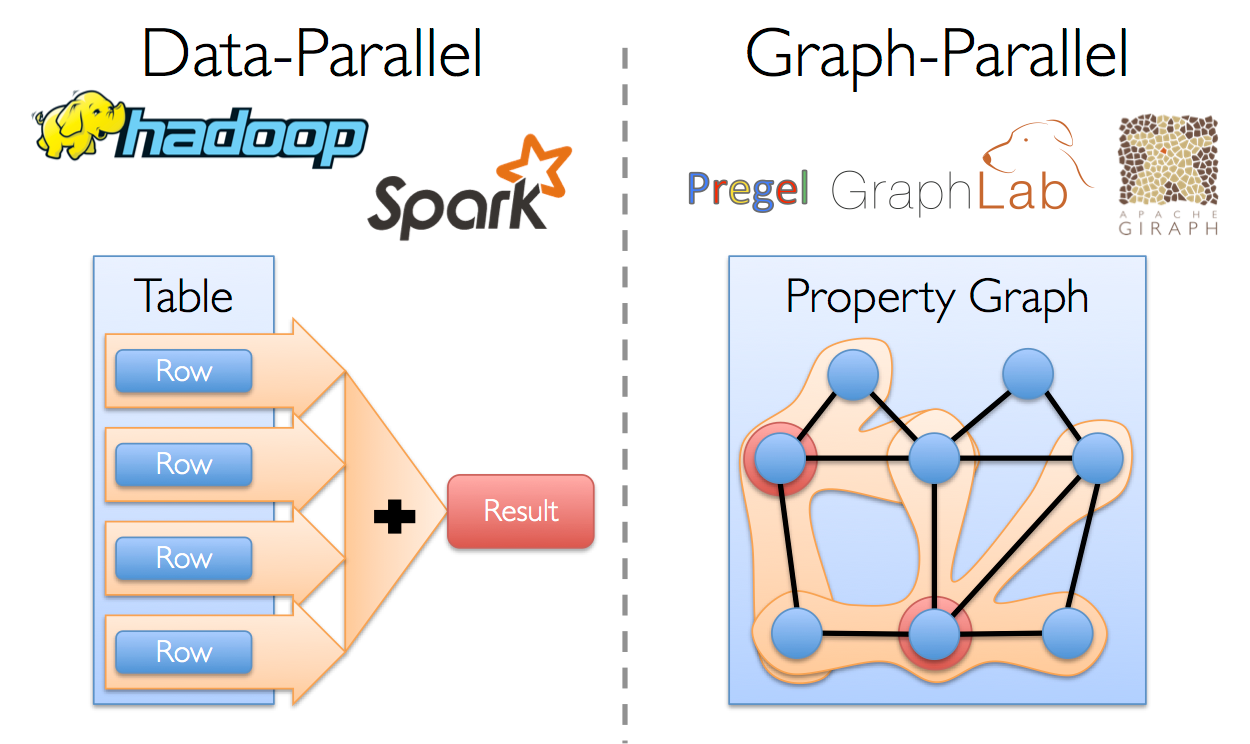
\includegraphics[scale=0.3]{images/image00}
\caption{Difference between data-parallel and graph-parallel}
\label{fig:parallel}
\end{figure}

Data-parallel systems like Hadoop, Spark, Beam, etc treats the data as sets of records and do the parallel processing. Graph-parallel systems treats the data as a graph, where data get mapped to nodes and edges to represent the relationships between data. See Figure \ref{fig:parallel}. Some examples for graph-parallel systems are Pregel, GraphLab.

\section{Big Data and Big Graph}
Big data is emerging as a hype these days as businesses has realised they can generate more revenue by analysing their huge piles of data and generating better business insights,  uncover hidden patterns, correlations. 

\paragraph{}

With the popularity of the Big Data, the idea of using graphs to uncover relationships of data has also emerged. Experts says it is “not about finding the right answer to a question but about seeking the right question to ask."\footnote{http://www.informationweek.com/big-data/big-data-analytics/graph-analytics-the-other-big-data/d/d-id/1109724} We see tools for analysing huge graphs are getting developed.

\section{Graph streams}
A graph stream is a stream of data which includes data about entities and their relationships, which we can map into a set of nodes and edges on a graph. For instance, "user001 liked image0004" can be mapped in to an edge where "user001" and "image0004" are nodes and these nodes are connected with an edge called "liked".

\section{Query Platforms}
Query platforms enables developers easily query data from the graph. We often see people use tools to run queries to fetch data on the fly. There are two main types of query platforms, some like Apache Giraph where they provide a programmatical interface\footnote{http://giraph.apache.org/apidocs/} and users have to write the code for the analysis process. 

\paragraph{}

Other type is, where they provide a query language and a query parser engine which convert the query written in query language to the analysis process. Different type of query languages introduced for different needs. Hive SQL\footnote{https://hive.apache.org/} and Spark SQL\footnote{http://spark.apache.org/sql/} are both for data-parallel systems while Gremlin\footnote{http://tinkerpop.apache.org/gremlin.html} is a query language in Apache TinkerPop stack which can be used for both graph databases (OLTP, Online transaction processing) and graph analytic systems (OLAP, online analytical processing).

\section{Graph partitioning}
Graph partitioning methods have to be accommodate to partition these generated massive-scale unbounded graphs to be assigned to  different computation nodes in order to do the analysis. Best partitions would be having less connections in between partitions, thus, will reduces the communication between partitions, which could be costly otherwise.

\subsection{Edge-cut and Vertex-cut methods}
Existing graph partitioning methods can be divided into two main categories, as edge-cut and vertex-cut methods\cite{S-PowerGraph}. Edge-cut tries to evenly assign the vertices to machines by cutting the edges and vertex-cut tries to evenly assign the edges to machines by cutting the vertices.
 
\subsection{Graph partitioning for Natural graphs}
However, the natural graphs commonly found in the real-world have highly skewed power-law degree distributions \cite{powerLaw1} \cite{powerLaw2}, which challenge the assumptions made by abstractions like  Pregel\cite{Pregel} and GraphLab\cite{Graphlab}, limiting performance and scalability. As natural graphs are highly skewed, there exists subset of vertices which have large number of edges. 

\paragraph{}

For example, a common World Wide Web crawler would find most of the web pages have average number of hyperlinks pointing to them while some web pages have massive number of hyperlinks pointing to them, we call these web graphs\cite{WebGraphs}. 

\paragraph{}

When we use edge-cut approach evenly distributing vertices could result some partitions with too many edges but when we use vertex-cut approach we get edges evenly distributed across the partitions, therefore no one partition would get too much load. Therefore, vertex-cut methods can achieve better performance than edge-cut methods\cite{PowerGraph} specially for graphs that follows power-law degree distribution.

\subsection{Optimal partitioning}
	An optimal partitioning means where the communication between partitions to perform a computation is minimal and the needed computation power and storage are balanced across the partitions.

\section{Graph Analysis Frameworks}
We started analysing the currently available graph analysis frameworks to understand their internal workings, how they handle large scale graphs, queries, etc. These frameworks usually falls into two categories, as
\begin{enumerate}
\item OLTP (Online Transaction Processing)
\item OLAP (Online Analytical Processing)
\end{enumerate}

Online Transaction Processing frameworks are graph databases characterized by a large number of short online transactions (INSERT, UPDATE, DELETE). Online Analytical Processing aggregated are graph databases with historical data, stored in multidimensional schemas and characterized by relatively low volume of transactions. Research interest of this research is towards Online Analytical Processing rather Online Transaction Processing. Therefore, we evaluated currently available OLAP frameworks here.

\paragraph{}

Most of the well known solution in the literature and industry are only capable of analysing graphs that no new vertices or edges are added to the graph over the time\cite{Pregel} \cite{Graphlab}. These type of graphs are called bounded graphs while the graphs where new vertices and edges are inserted  over the time are called unbounded graphs or streaming graphs\cite{Fennel}\cite{S-PowerGraph}. 

\paragraph{}

Several of these solutions allow changing the graph structure, that is, how edges are connected to the vertices. These dynamically changing graphs are called dynamic graphs and others are called static graphs, where the graph structure does not change\cite{X-stream}.

\paragraph{}

We evaluated several such graph analysis frameworks to identify their strengths and weaknesses. You can find our findings under Appendix A.

\paragraph{}

Almost all the solutions use some kind of graph partitioning techniques. We will be discussing some of the available graph partitioning techniques in the next section.  

\section{Graph Partitioning algorithms}
In graph-parallel systems, the graph is partitioned into several sub graphs across processing resources for two main reasons, first, one huge graph might not fit in one, second, if we can distributed a graph on several computational nodes, then we do the processing parallelly and get the expected results quickly.  

\paragraph{}

Almost all the solutions above use graph partitioning techniques to parallelize the computations. Some key aspects considered in graph partitioning is how to minimize communication and how to balance computation and storage. 

\paragraph{}

We evaluated several graph partitioning techniques to get an insightful understanding on graph partitioning, to evaluate their strengths and weaknesses. You can find them under Appendix B. 

\section{Graph summarization}
Graph summarization is an interesting area of graphs where we create a summary of a huge graph. We can then do our computation on the summary instead of the original graph, but what we get is an approximate result. 

\begin{figure}[H]
\centering
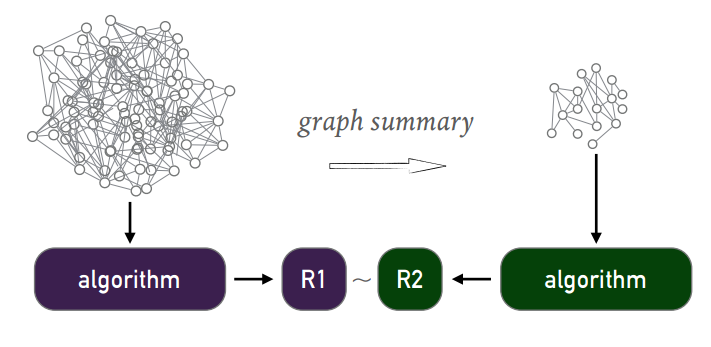
\includegraphics[scale=0.6]{images/image02}
\caption{Graph summarization and result approximation}
\end{figure}

\paragraph{}
Some highlighting properties of graph summarization are, 

\begin{enumerate}

\item $ | S_G | << | G |$ : the size of sketch $S_G$ is far less than the graph G, preferably in sublinear space.
\item The time to construct $S_G$ from G is in linear time.
\item The update cost of $S_G$ for each edge insertion/ deletion is in constant time.

\end{enumerate}

Some example sketching techniques are frequency counts\cite{frequency counts}, Count-Min\cite{CountMin} and its variant gSketch\cite{gSketch}. But them both can support only a limited types of graph analytics, since they are not graphs.

\begin{figure}[H]
\centering
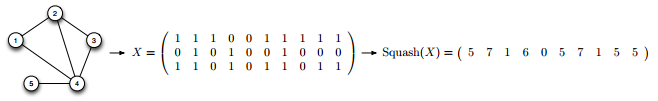
\includegraphics[scale=0.6]{images/image15}
\caption{Count-Min's sketching technique visualized}
\end{figure}


\paragraph{}

We evaluated several available graph summarization techniques in the literature and among them were different spanners\cite{sparse spanners}, sparsifiers\cite{Spectral sparsification}  and sketchers techniques. \cite{Graph stream algorithms survey} is a survey on these techniques.    

\subsection{Frequency Counts}
Frequency Counts\cite{frequency counts} is a simple sketching technique over graph stream. It create two separate sketches for nodes and edges as you can see in the Figure \ref{fig:NodeSketches} and Figure \ref{fig:EdgeSketches} which are sketches of a sample graph stream in the Figure \ref{fig:SampleGraphStream}

\begin{figure}[H]
\centering
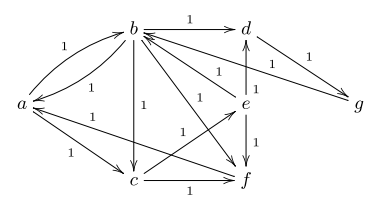
\includegraphics[scale=0.6]{images/SampleGraphStream}
\caption{A sample graph stream}
\label{fig:SampleGraphStream}
\end{figure}

\begin{figure}[H]
\centering
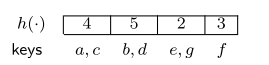
\includegraphics[scale=0.6]{images/NodeSketches}
\caption{Node Sketches}
\label{fig:NodeSketches}
\end{figure}

\begin{figure}[H]
\centering
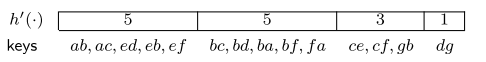
\includegraphics[scale=0.6]{images/EdgeSketches}
\caption{Edge Sketches}
\label{fig:EdgeSketches}
\end{figure}

Frequency Counts lacks the ability to respond to connectivity queries as the connectivity of the graph is not preserved in the sketches\cite{TCM}.

\subsection{TCM}

TCM\cite{TCM} introduce a graphical sketch where a graph $S_G$(V, E), where V denotes the set of vertices and E its edges, is the summary of the graph G(V,E) and $|S_G| << |G|$. TCM promises a graph analytical method M which needs to run over a graph stream G, denoted as M(G), one can run it directly on its sketch $S_G$, M($S_G$), to get an approximate result, without modifying the method M.

\begin{figure}[H]
\centering
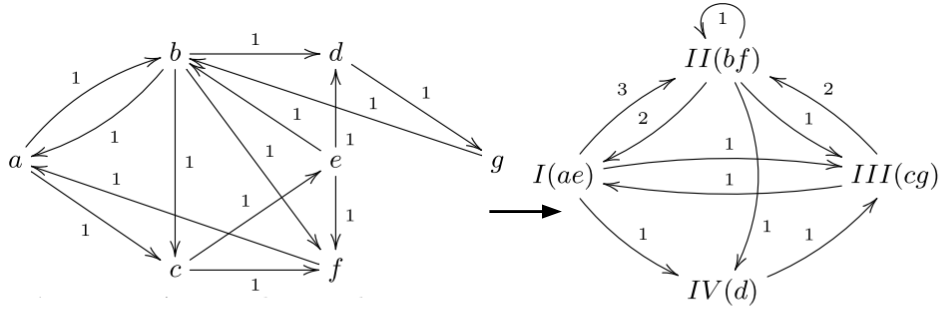
\includegraphics[scale=0.3]{images/graph-sketching}
\caption{Example TCM sketch for a graph}
\end{figure}

\paragraph{}

In the TCM model, a sketch denotes an adjacency matrix of size m, which is called the sketch size. A set of such sketches are maintained, and when queried for information, the query is run on all the sketches simultaneously and the results from each sketch is merged to produced the final output. Merging the results of the sketches is done by using a aggregation function, which could be min(), max(), count() or any other. 

\paragraph{}

That is, for a given graph analytic method M to run on G, that is M(G), it is possible to run M on each n sketch separately, and then merge the result as follows, where $\tilde{M}(G)$ is the estimated result over G, and $\Gamma()$ is an aggregation function 

\paragraph{}

\begin{equation}
\tilde{M}(G) = \Gamma(M(S_1), ......., M(S_n))
\end{equation}

When an edge query is given, which can be denoted as $f_e(a,b)$ where a and b are node ids, the resulting approximated value, which is denoted as $\tilde{f}_e(a,b)$, could be calculated like as follows.

\begin{enumerate}
\item First  estimate edge weight $M_i[h(a)][h(b)] $ where $M_i[h(a)][h(b)]$ is the cell value relative to position h(a) and h(b) in adjacency matrix $M_i$ and h is the hash function.
\item Then uses a corresponding function $\Gamma()$ to merge the values from each matrix $M_i$.
\end{enumerate}
 
We can denote it as follows, 

\begin{equation}
\tilde{f_e}(a,b) = \Gamma(M_1[h(a)][h(b)], ......., M_n[h(a)][h(b)])
\end{equation}

You can see that estimating the aggregate weight of an edge query is in O(n) time, where n is a constant.


\chapter{Preliminaries of querying for streaming graphs}


\section{Graph analysis frameworks}
We started analysing the currently available graph analysis frameworks to understand their internal workings, how they handle large scale graphs, queries, etc.

\paragraph{}

Most of them like Pregel\cite{Pregel} and GraphLab\cite{Graphlab} are only capable of analysis bounded graphs and some of them like X-stream\cite{X-stream} were not able to handle dynamic graphs and only supports static graphs. 

\section{Graph partitioning}
One reason for this is graph partitioning played a significant role in almost all of them and effective graph partitioning is easy only when the whole graph can be seen. But the problem with unbounded graph is, only a part of the graph, that is the part that has received already and without seeing the rest of the graph, can’t guarantee an optimal partitioning.
 
\paragraph{}

We looked into streaming partitioning algorithms in the literature. Streaming partitioning algorithms uses heuristics\cite{Streaming Balanced Graph Partitioning Algorithms1} \cite{Streaming Balanced Graph Partitioning Algorithms2} to assign vertices and edges to the partitions. Something noteworthy is, if it is possible to partition an unbounded graph using one particular streaming partitioning algorithm, then the same algorithm could be used to partition a bounded graph. The reason is, a bounded graph can be streamed as an unbounded graph.
 
\section{Streaming graph partitioning}
We then studied about many streaming graph partitioning techniques and observed most of them are considering about the adjacency and balanced partitioning. Some of them focus on properties of natural graphs and trying to exploit them when partitioning. We studied on the natural graphs and their properties to get a clear understanding on how we can use them for efficient partitioning. 

\paragraph{}

One problem with graph partitioning  is that when a computation was performed on the graph, there happens lot of inter-partition communications. For instance, when running PageRank on the graph, a node which has a neighbour in another partition has to communicate with that partition to get its current PageRank. Usually there exists many such vertices and one such vertex may connect to many other neighbours which resides in other partitions. This results in many messages passed in every iteration of the PageRank algorithm. There are many such queries which needs lot of inter partition communications happen to generate the final output.

\paragraph{}

A graph stream of a natural graph was needed to carry out some initial evaluations. Therefore we started implementing a Twitter stream listener, where we can listen to the Tweets the Tweeters Tweet at any given moment in real-time as a data stream. Our plan was to map the data stream into a graph stream and then start building a graph. 

\paragraph{}

We were evaluating the Spark and Flink frameworks by the time. We first evaluated the possibility of implementing this with GraphX, Spark’s graph framework, then comprehended GraphX is not capable of handling unbounded graphs. Then we moved on to Flink’s graph analysis framework, Gelly. 

\paragraph{}

Same as GraphX, Gelly also was only for unbounded graphs, however, we came to know with some more digging in, there is an ongoing research\cite{Kalavri} to extend Gelly to support unbounded graphs. That was by a research team from KTH, Royal Institute of Technology, Stockholm, Sweden and they have a working prototype\footnote{https://github.com/vasia/gelly-streaming}. However, they do not build a graph from the graph stream, instead use one pass algorithms to just filter out the informations they are interested in. 


\section{One pass algorithms}

One pass algorithms are a type of algorithms which reads its input exactly once, in order, without unbounded buffering. Some simple use cases of one pass algorithms are counting the elements, seeking the k largest or smallest elements, finding the sum, mean, variance and standard deviation of the elements, finding the most or least frequent elements, etc. 

\paragraph{}

However, the problem with one pass algorithms is that it is not a general way to run all the graph analysis types we know. We have to know the one pass algorithms or invent new ones for our analyses. 

\paragraph{}

What they have done in their research is implementing the known algorithms, like Connected Components, Continuous Degree Aggregate, etc. They provide some basic set of operations over the graph stream like aggregation, transformations, slicing into windows, etc. But graph specific operations like traversing the neighbours are available only within a window as they don’t maintain a graph. They are using the shared states to continue the extracted information across the stream.

\section{Graph summarisation}

What we wanted is a more general method, where the users can perform any type of graph analysis on our platform, which is not possible with one pass algorithms. We then sought for other solutions and came across graph summarisation. The goal of graph summarisation is to produce a compressed representation of a graph. 

\section{Spanners, sparsifiers and sketches}

Among several summarization techniques, spanners which is for distance estimation, sparsifiers which is for cut estimation and sketches which is for homomorphic properties are the highlighting ones. We started studying about spanners, sparsifiers and sketches. \cite{Graph sketches} and \cite{Graph stream algorithms survey} discusses on different scenarios where we can use spanners, sparsifiers and sketches.

\paragraph{}

Spanners and sparsifiers were left out as they were used mainly for distance estimation and cut estimation, and what needed was something which can represent the properties of original graph as a summary, not just distance or cuts.

\paragraph{}

The problem with sketching is, like one pass algorithms, sketching are also query specific. However, TCM sketching promises the ability to use in general. 

\section{TCM sketching}

TCM introduces a sketching technique which can be used to all types of graph analysis queries in general. In the TCM paper they have shown how TCM enables to run all 4 types of graph analysis queries, which are nodes queries, edge queries, path queries and subgraph queries. 

\paragraph{}

We then implemented TCM sketching as a standalone Java application. More information on implementation could be found under next chapter.

\chapter{Querying for streaming graphs}
\section{Evaluating TCM}

We then wrote a web crawler which crawls the world wide web and create a graph stream about web pages and their links to other web pages. This graph stream used to continue with our testing on TCM. 

\paragraph{}

Visualizations of the building original graph and the sketches were created using a visualisation framework in order to get an idea. Several sketches with several sizes were created and visualized. Then started running different type of graph analysis queries on the sketches. 

\section{Dynamic querying}

However, our system had one limitation, that is, whenever wanted to run a new query the running process of building the graph had to be stooped and rerun changing the query. Then the graph starts building from the beginning which takes a lot of time, specially to become a  natural graph, showing power-low degree distribution. 

\paragraph{}

We followed two approaches here, one is we wrote our TCM implementation as a OSGi bundle, where we can keep the graph building and run any query on it dynamically, attaching to the graph. More about this could be found under next chapter. 

\paragraph{}

This way, we firstly deploy the TCM graph as a OSGi bundle to the OSGi platform and then we can submit a query as a OSGi bundle to the OSGi platform. OSGi bundles are compiled into JAR files, which we can dynamically load to the OSGi platform. 

\section{Simulation}

Other approach was to use Snapy.py which is a graph generation library by Stanford and generate a stream of graph and build the sketches.  With Snapy.py we can generate different types of graphs and with different degree distributions. This way, we could generate and analyse both random and natural graphs.


\paragraph{}

Number of sketches and the size of the sketches, that is the dimensions of the adjacency matrix of the sketch has a relation between how accurate the local and the final result for the analysis. Therefore, we tried generating different sketches, with different sizes and different number of sketches and continued to analyse the accuracy. 

\paragraph{}

We used a node query and plotted degree distribution of the vertices of the original graph and then used the same node query and plotted degree distribution of the vertices from the sketches. We then could compare the two plots to get an idea on the effects of sketches on the accuracy.  Then we performed a series of evaluations with TCM sketching. 

\section{Extending TCM}

One problem we understood with the TCM sketching was, we have to define the sketches beforehand. However, when working with the unbounded graphs, we don’t know how large the graph would grow. Because there is an relation between accuracy and number of sketches and sketch sizes, we saw the accuracy degrades when the graph is getting bigger. 

\paragraph{}

How TCM paper discuss to create a sketch is to take the full memory of the computation unit it is built on and create a sketch of that size and number of computation units available is how many sketches we create. However, when the graph is getting bigger, the accuracy keeps degrading. 

\paragraph{}

Creating a sketch of the size of the available memory is not a good solution in an era of cloud computation and distributed computing. We today is capable of vertically and horizontally scaling the resources available and pay as of the usage. We could start with 2GB of memory on one unit and scale up to 2TB of memory on 100s of units each.

\paragraph{}

As a graph analysis framework we have to handle this. This is a significant point where we have to come up with a novel idea to introduce extensions to the TCM model for automatic sketch creation. Thus we started investigation on this.

\paragraph{}

First we had to clarify what we consider as accuracy because definition of the accuracy is vague and changes with the type of the query. However, when looking at the fundamentals, we realized, the factor which relates to the accuracy of a TCM sketch is how many nodes of the original graph maps to a node of the sketch.

\paragraph{}

 For example, if the nodes of the original graph is as G[a,b,c,d,e,...] and nodes of sketch is as S[I, II, III, IV, ...,], when  we have only one node of original graph mapped to one node of sketch, as S[ I(a), II(b), III(c), IV(d),...], then the sketch is same as the original graph, whatever the query we run on sketch gives same results as the original graph. But when two nodes of the original graph shares one node of the sketch, as S[ I(a,e), II(b), III(c), IV(d),...], the accuracy might degrade. When more different nodes of the original graph maps to one node of the sketch is when the accuracy starts to fall.
 
\begin{figure}[H]
\centering
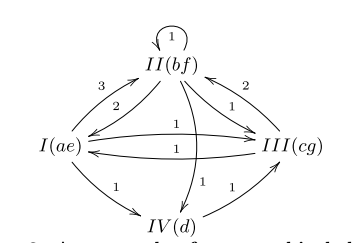
\includegraphics[scale=0.6]{images/example-tcm}
\end{figure}

\paragraph{}

 However, when we create different sketches using pairwise independent hashing,  nodes of the original graph which mapped to one node of a sketch, get distributed to other nodes of another sketch. This again increases the accuracy. 

\paragraph{}

The main two problem was identifying when to create a new sketch and how to create a new sketch just by looking at the existing sketches. Since we hash the nodes to put into the sketches we have no way of reversing the hash and hashing again to the new sketch.

\paragraph{}

For example, let us say we have an edge like (u,v) and two sketches as S1 and S2 having adjacency matrices as M1 and M2 with sizes as 9 and 17 respectively.. When we insert the edge to S1 it hash both the vertices for the range of 0 to 9 and we got values 2,4 respectively. Now, we can put this edge to the sketch S1  by incrementing the value at M1[2][4]. 

\paragraph{}

If we insert the edge to S2 it hash both the vertices for the range of 0 to 17 and and say we get values 5,11 respectively. Now, we can put this edge to the sketch S2  by incrementing the value at M2[5][11]. But when we want to put the vertices mapped to M1[2][4] into S2’s adjacency matrices M2 and if we don’t have the original vertices at hand, we have no way of knowing  to which values these vertices maps in the S2’s adjacency matrices M2.

\paragraph{}

We thought about considering above two factors, number of average overlapping nodes( N ) and number of sketches( S ), and keeping them to a ratio ( like  k  ∝ N/S ) to keep the accuracy at a fixed rate, because if we consider graph density is proportional to the average overlapping nodes, we can easily calculate this and can empirically evaluate this.

\paragraph{}

However, we realized we can solve our two main problems, when to create a new sketch and how to create a new sketch by looking at values returned from the sketches. For example, let's say we have 4 sketches with sizes as a, b, c, d where a \textless  b \textless c \textless d. When we query for an edge, each sketch returns the edge value as of that sketch and  we put these values to a list like this [ 7, 4, 3, 3 ] for instance, then what we do is, get the minimum value from the list, assuming it is the correct value and return as the result of that query.

\begin{figure}[H]
\centering
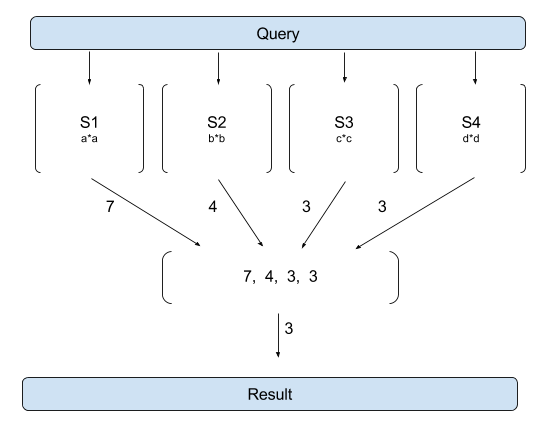
\includegraphics[scale=0.7]{images/QueryOnSketches}
\caption{Querying happening on the sketches}
\end{figure}

\paragraph{}

At the beginning, for a given edge, the sketches might return something like [ 3, 2, 2, 2 ], but when the graph is growing, the smaller sketch will get more hash collisions, thus will return something like this, [ 7, 4, 3, 3  ]. We can understand looking at this, even though the correct value is 3 here, we have one sketch which gives the value as 7. When we see something like this, where some sketches are deviated from the correct value( minimum value ), then that is the correct time to create new sketches. 

\paragraph{}

We don't have to run edge queries for this explicitly, because when we insert an edge, we already query for the edge first to get the current value, 

\begin{algorithm}
\caption{Adding a new edge to a sketch}
\label{alg1}
\begin{algorithmic}
\STATE
\STATE $edgeValue \leftarrow m[a,b] $ 
\STATE $m[a,b] \leftarrow edgeValue + 1 $ 
\STATE
\end{algorithmic}
\end{algorithm}

This means we do not add overhead to the system and reading edge value is a constant time operation because what we do is read the adjacency matrix. 

\paragraph{}

When we think further, we thought we can delay creating a new sketch until it is only one sketch out of all sketches that return the correct value. We did several experiments on this, you can find the results under Results and Evaluation section.

\paragraph{}

Once we know when to create a new sketch, next problem we get is how to create a new sketch. Then we investigated how can we create new sketches using the knowledge we have at hand and we saw we can do it at the same time while checking whether we have to create a new sketch.

\paragraph{}

Let’s say while inserting an edge,  we decide to create a new sketch by looking at sketch values. We first create a new sketch with larger size and fill it with Nulls ( ∅ ). Let’s says  the sketch values were like this [ 7, 4, 3, 3 ]. From this sketch values we get the correct value as 3 and we can set the new sketch's value for that edge as 3, making the final sketch values list as  [ 7, 4, 3, 3, 3 ]. 

\paragraph{}

The next time we get an another query, we might get something like this for sketch values, [ 9, 3, 2, 2, ∅ ] because we have a new sketch and its matrix is filled with ∅s mostly. Now we omit the ∅ and get 2 as the correct value and then we set the new sketch’s adjacency matrix’s corresponding cell with that value. This way, we eventually fill the new sketches with very less overhead.  

\paragraph{}

We implemented this automatic sketch creating mechanism and tested for the accuracy with different measures. We firstly passed an array of sketch sizes in ascending order as parameters and let the sketches create automatically, but using the first two sketch sizes as the starting sketches. Then we identified how many sketches used by the system to store the given graph stream. Then we did the experiment giving the same graph stream but instead of creating the sketches dynamically, we created the the same number of sketches with the same sketch sizes at the beginning, like previous experiments.

\paragraph{}

Then we compared the outputs against the original graph and against each other. Then we compared the created sketches in both mechanisms and calculated how the sketches has deviated in the auto sketch creating technique  than the non auto sketch creating technique. You can find more details on this under the Results and Evaluation chapter. 

\paragraph{}

In this experiment the program waited until it is just one sketch that is giving the right value to create a new sketch as we described above. We could use several other techniques like this. We see these as automatic sketch creation policies. We tried several such policies and the evaluated the results. 

\paragraph{}

Some such policies we tried are, without waiting until it is just one sketch giving the correct results, we tried with waiting until it is only 2 sketch giving the correct results, only 3 sketches giving the correct results, half of the sketches giving the correct results, ¼ of the sketches giving the correct results, etc.  You can find more details on this under the Results and Evaluation chapter.

\paragraph{}

Then we tried tolerating errors upto a limit, that is, when there is only one sketch giving the correct result, say ‘v’, we checked how many sketches are having ‘v+1’ as the sketch value. If we have one or more sketches giving ‘v+1’, then we do not create a sketch. This is useful when we do not need exact values to be in sketches, but something very approximate. We call this the tolerance, where 1-tolerance means if the correct value is ‘v’ but when we have a ‘v+1’ in the sketch values we do not create a new sketch, and 2-tolerance means we do not create a sketch when we have a ‘v+1’ or ‘v+2’ in the sketch values. In our implementation we defined n-tolerance where the user can define the tolerance they need. 

\paragraph{}

We can have tolerance with different policies, like  only 2 sketches giving the correct results + 2-tolerance. Then the system check if at least 2 sketch values have either ‘v’ or ‘v+1’ or ‘v+2’ if the correct value is ‘v’. We did a series of tests with different combinations and evaluated the accuracy of the queries. You can find more details on this under the Results and Evaluation chapter.

\paragraph{}

Since we are building a framework, we should give the users to choose which policy suits for them. Therefore, in our implementation, we have a parent class as ‘SketchCreationPolicy’ and several sketch creation policies implemented as child classes of it. This way, the user can use whatever the sketch creation policy they like when setting up the graph or write their own sketch creation policy by extending the ‘SketchCreationPolicy’ class. More on this can be found under the Implementation chapter.


\paragraph{}

We have a problem when creating the initial sketch or sketches as we lacks knowledge on the graph stream's velocity, that is how many edges get inserted in a unit time. The solution we used is to listen to the stream for a time and count the edges and nodes we see within that time. We then multiply the number of nodes into a scaling factor and use that size as the initial sketch size. The time and the scaling factor is configurable in the system.

\paragraph{}

\section{Optimising the operations}
We analysed our design looking for improvements, to understand where we can optimise. We saw three types of operations we do on sketches.

\begin{enumerate}
\item Reading the value of the adjacency matrix giving a row and a column ids.
\item Summing the values along a row of the adjacency matrix to calculate the outgoing edges 
\item Summing the values along a column of the adjacency matrix to calculate the incoming edges
\end{enumerate}


\paragraph{}

Reading the value of the adjacency matrix given a row and a column ids is constant time operation. However, summing the values along a row of the adjacency matrix to calculate the outgoing edges or summing the values along a column of the adjacency matrix to calculate the incoming edges is a O(m) operation on a MxM adjacency matrix.

\paragraph{}

However, we can update the sum of the row and the column with every edge insertion in constant time, by keeping a separate list of sums. This is like having M+1 rows and columns in the adjacency matrix, where the additional row and column keeping the sums. We tried this and evaluated the performance gain when querying. 

\section{Persistence}
User might want to shutdown the system and restart later or may want to take backups time to time in any case of system crash. We should provide a way to persist the graph in the memory onto a persistent storage. 

\paragraph{}

What we have in memory is a set of adjacency matrices, that are 2d matrices and some meta data.  In our design, we have a persistence interface where we can plug an adaptor for any persistence method. 

\paragraph{}

One such easy way is dumping to a text file.  We implemented an adaptor to dump the sketches along with its metadata to a text file in both JSON and XML formats. An another convenient way we can persist the sketches is to use a database. However, we can’t fit the sketches to a relational database as there are no fix column sizes for sketches. Therefore, we have to go with a NoSQL database where there are no schemas. After some study on available NoSQL systems, we identified document family databases like MongoDB would be easily used for this. We developed an adaptor to persist the sketches along with the metadata into a MongoDB instance.

\paragraph{}

We see that while we are persisting the sketches, we get new edge insertions as this persisting process takes some time. Here we implemented two versions of persistence, one is blocking and other is non-blocking. In blocking persistence, we hold new edge insertions until the sketches are persisted. In non-blocking persistence we allow new edge insertions. However, we firstly create a separate copy of the sketches, like a snapshot,  in the memory by memory copying, and then use that snapshot for persisting. Java has a native method to create a copy of an array from memory block copying. 

\paragraph{}

In the same way, we implemented a restore functionality where we can load the sketched persisted in any of the above methods into the memory and then continue building those sketches thereafter.

\chapter{Results and Evaluation}
In this chapter, evaluation of the proposed model, the results and the important parts of the implementation are discussed. Java was chosen as the implementation language as of the vast set of tools available and abundance community and references.

\section{High level architecture}

\begin{figure}[H]
\centering
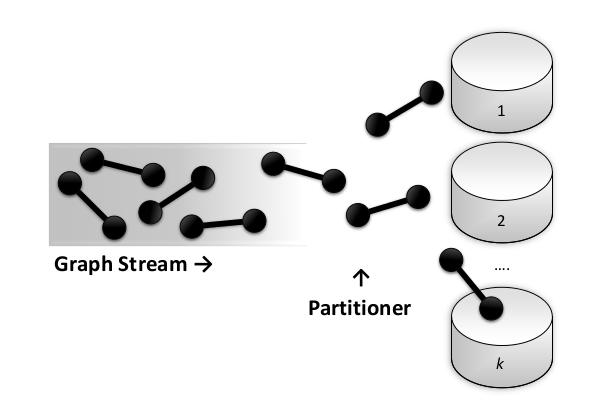
\includegraphics[scale=0.7]{images/image01}
\caption{High level architecture}
\end{figure}

\subsection*{Graph stream interface}
The users should be able to plug a stream of data to the systems, then a mapper which maps data into edges and vertices and input to the graph model as a graph stream.

\subsection*{Graph model}
Graph model is how the graph represented in the memory and in this proposed system graph sketches are used for this. 

\subsection*{Graph sketching}
There are many sketching techniques, some techniques limits the model for specific types of queries. This research used TCM sketching model as the sketching technique as it is a general purpose sketching technique.

\subsubsection*{Sketch creation}
As the graph build over the time, new sketches are created according to the used sketch creation policy in order to preserve the accuracy at a reasonable level.  

\subsubsection*{Sketch deletion}
As new sketches with higher sizes are created,  the small sketches are removed when their contribution to the accuracy decrease.

\subsection*{Persistence interface}
The interface where the sketches could be back-upped and restored.

\section{Abstract Class Diagram}

\begin{figure}[H]
\centering
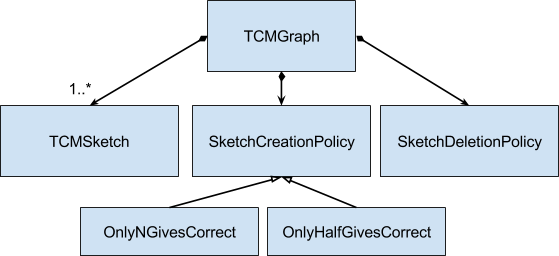
\includegraphics[scale=0.8]{images/image06}
\caption{Abstract Class Diagram}
\end{figure}

\section{Graph summaries}
When implementing the adjacency matrices of the sketches, a Java 2D arrays was used, as the array sizes are known  beforehand and the operations which are performed on them are only setting and getting array values by giving the array indexes and this operations takes constant time on array data structures.

\paragraph{}

For the sketch value list where the values returned by the sketches are kept, an array was used initially but later moved to a heap. Retrieving the minimum values was the mostly performed operation on this list.  With array, we could get the sketch id of the minimum values by its array index. 

\paragraph{}

But later, a class called "SketchValue" was defined, which holds the value returned from the sketch, sketch id, sketch creation time and sketch confidence. Then instances of these "SketchValue" are stored on the heap. 

\paragraph{}

The reason to have a such "SketchValue" class was, this list of "SketchValue"s are passed to the Sketch Creating Policy and Sketch Deletion Policy, and the additional information such as sketch creation time and sketch confidence can be used by these policies to decide if a new sketch should be created and if a particular sketch should be deleted.
 
\section{OSGi bundles}

Dynamic service deployment was needed to submit queries on the fly to dynamically query the graph time to time and Apache Felix was used as a OSGi Framework and Service platform as it is an open source project. 

\begin{figure}[H]
\centering
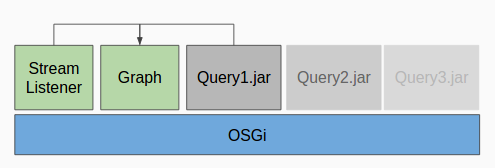
\includegraphics[scale=0.6]{images/OSGi}
\caption{Dynamically submitting Query jobs on OSGi platform}
\end{figure}

Here the Stream Listener listen to the data stream, map the stream to a graph stream and insert into the graph. One or more Stream Listeners can be attached to a graph where more than one stream contributes to the graph. Then Query Jobs can we submitted to the OSGi platform as OSGi bundles which comes as JAR files. Though the CLI of the OSGi platform, we can manage these submitted Query jobs, add new jobs, view running jobs, stop running jobs, etc. The Query get attached to the graph and retrieve the necessary information for the analysis. 

\section{Natural graphs from Webcrawler}
Following is a web graph generated by mapping the data stream of our web crawler as a graph stream and then built the graph. Each node indicates a webpage on the World Wide Web and each edge indicates a hyperlink between two such webpages. You can see some nodes having many hyperlink while some have only few. 

\begin{figure}[H]
\centering
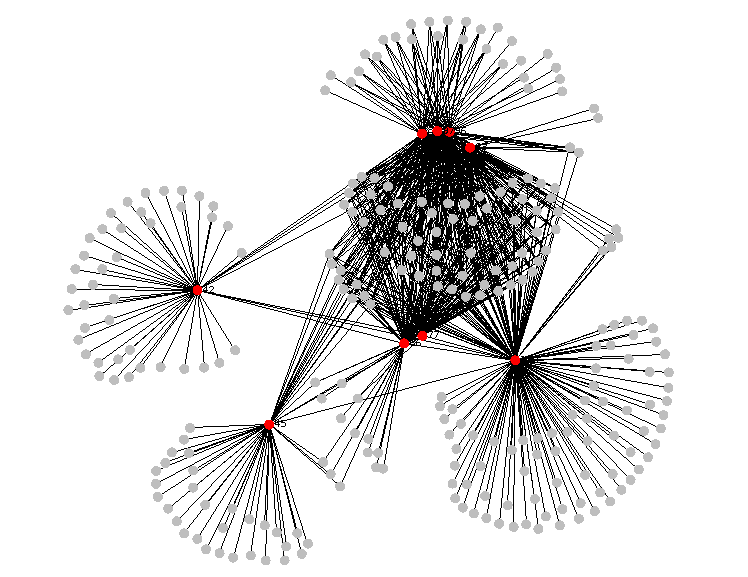
\includegraphics[scale=0.6]{images/web-graph}
\caption{A large web graph generated by our web-crawler}
\end{figure}

It took us about half an hours to build this graph because crawling the web and fetching the hyperlinks from the webpage’s contents by parsing the HTML is a time consuming task. 

\paragraph{}

Following is a also as above graph, but a zoomed out view and with many more nodes. The red dots you see are actually groups of nodes connected together. Edges has been removed for clarity but you can get an idea about the connectivity of nodes by the closeness of the nodes. You can see there are some nodes which has very high connectivity, thus forming big groups, as the one in the top left corner. 

\begin{figure}[H]
\centering
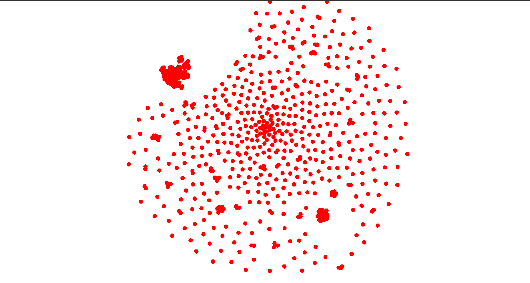
\includegraphics[scale=0.8]{images/graph2}
\caption[Zoomed out view of a large web graph]{Zoomed out view of a large web graph generated by our web-crawler}
\end{figure}

\section{TCM Sketching}
While creating the above graph, three sketches were created, but with very small sketch sizes, only to get a visual representation of the sketches. First one is a sketch of size 12. The second one is a sketch of size 33. The last one is a sketch of size 112.


\begin{figure}[H]
\centering
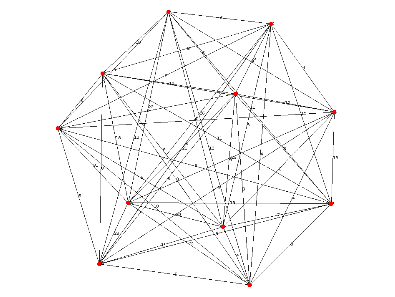
\includegraphics[scale=0.8]{images/s1}
\caption{A sketch of size 12}
\end{figure}



\begin{figure}[H]
\centering
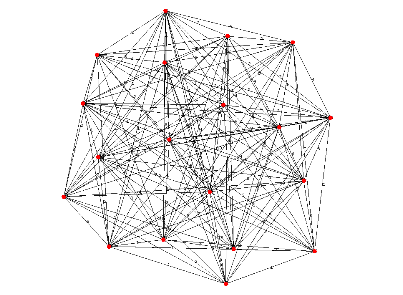
\includegraphics[scale=0.8]{images/s2}
\caption{A sketch of size 33}
\end{figure}

 

\begin{figure}[H]
\centering
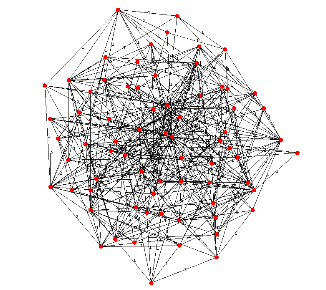
\includegraphics[scale=0.8]{images/s3}
\caption{A sketch of size 112}
\end{figure}

Next move was to use the sketches and query the graph. TCM paper has defined 4 types of queries and evaluated with several experiments. Node queries were chosen to start with as interesting queries like identifying top-k heavy hitters\cite{HeavyHitters}, conditional heavy hitters\cite{TCM}, etc are based on node queries, and then the edge queries are also evaluated.

\paragraph{}

We used small to medium scale graphs for initial testing, which ranges from 100 to 10,000 nodes and 1000 to 1,00,000 edges.  We did series of investigations using the graphs generated with Snapy.py using different configurations in generating graphs and sketches.

\paragraph{}

The most simplest node query is to ask the degree of a node giving a node id. What the experiment followed was, instead of asking random nodes, every node’s degree was asked by issuing series of node queries and using that information, calculated the number of nodes which has a certain degree. This way a degree distribution of the graph could be plotted. The same was queried from the original graph and was plotted the same.

\paragraph{}

Following is a degree distribution plot of a graph with 100 nodes and 1000 edges. The dotted line indicate the correct degree distribution which is calculated from the original graph, while the line indicates the degree distribution calculated by querying the TCM sketches. Here have used sketches of sizes 73, 79, 83, 89. You can see, there is a slight deviation between the two graphs but the original shape is preserved. 

\begin{figure}[H]
\centering
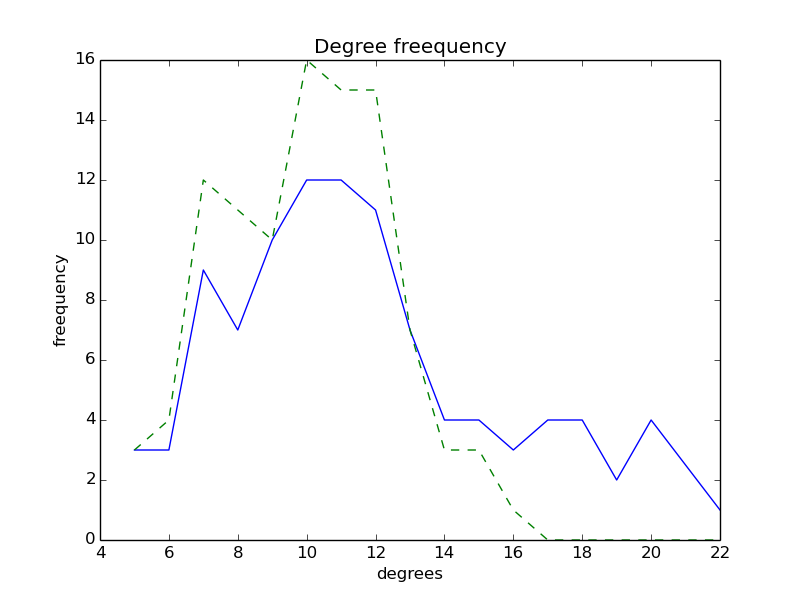
\includegraphics[scale=0.6]{images/dd1}
\caption{Degree distribution from sketches of sizes 73, 79, 83, 89}
\end{figure}

You can see a drop in the low degrees and a rise in the high degrees. This happens because of the small sketches having nodes which maps too many nodes of the original graph onto them, thus increasing the adjacency matrix’s corresponding cell value. When there are such nodes in the sketch, all the nodes of the original graph which maps to those nodes gives a higher values than they have. 

\paragraph{}

Next two graphs are the same as above but with sketches  of sizes 89, 97 and 83, 89, 97 respectively. You can see how the degree distribution plot drawn from the TCM sketches has become more closer to the degree distribution plot drawn from the original graph. The bigger size of the sketches has contributed to more accurate results comparing previous plot and next two plots. By comparing the next two plots you can see how more number of sketches has contributed to more accurate results.

\begin{figure}[H]
\centering
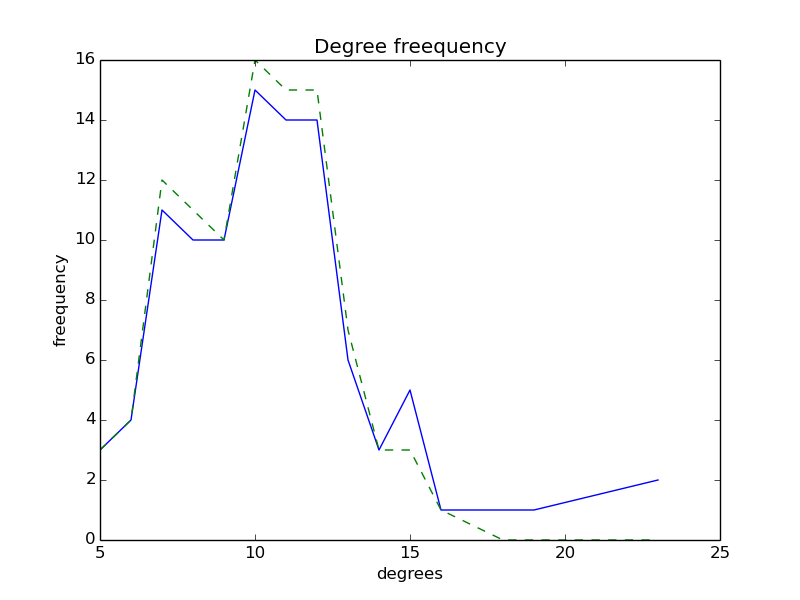
\includegraphics[scale=0.6]{images/dd2}
\caption{Degree distribution from sketches of sizes 89, 97}
\end{figure}

\begin{figure}[H]
\centering
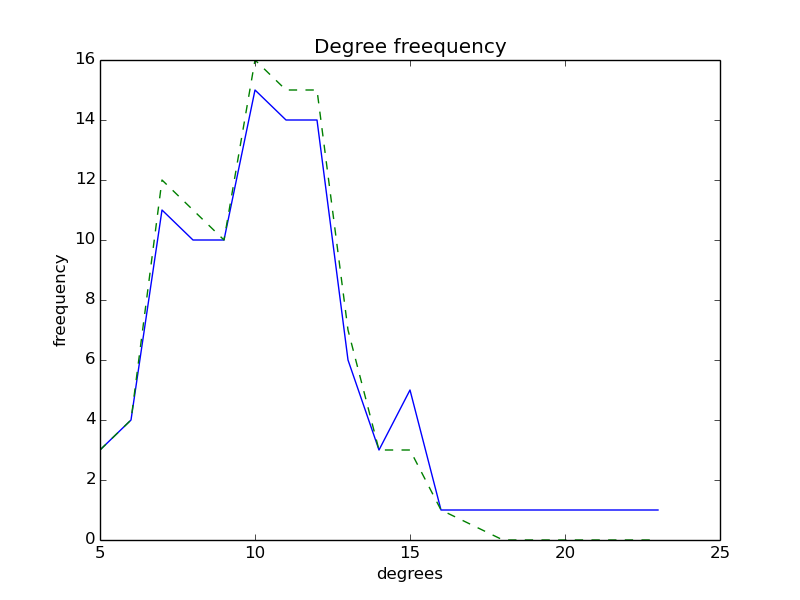
\includegraphics[scale=0.6]{images/dd3}
\caption{Degree distribution from sketches of sizes 83, 89, 97}
\end{figure}

\section{TCM Sketching for Natural graph}
Following is a plot of degree distribution of a natural graph, which was generated from our web crawler. The experiment time to time plotted the degree distribution of the graph by querying the sketches and from the original graph. The blue line indicate the correct degree distribution which is calculated from the original graph, while the red line indicates the degree distribution calculated by querying the TCM sketches. Here we have used sketches on sizes 11 19 71. You can see, there is a slight deviation between the two graphs but the original shape is preserved.

\begin{figure}[H]
\centering
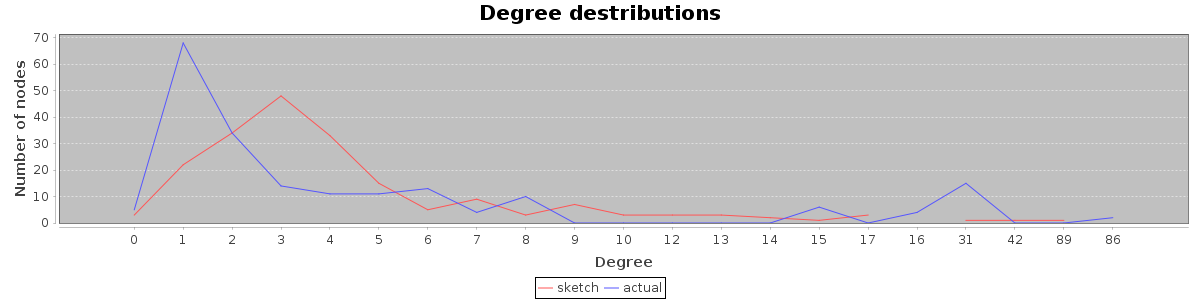
\includegraphics[scale=0.3]{images/ddn}
\caption{Degree distribution of a streaming natural graph from sketches of sizes 11, 19, 71}
\end{figure}

All the above experiments involved a series of node queries in each experiment and the results looked promising when visually compared. At this point, defining measures to evaluate the accuracy of the queries was needed. 

\section{Evaluation Metrics}
Number of queries running on the sketches giving the exact correct results as running on the original graph could be calculated easily, however, as the research is interested not only in exact correct results, but also in approximate results, this could not be used as a good measurement. Thus, better metrics were needed.

\paragraph{}

Average Relative Error and Number of Effective Queries was taken from gSketch\cite{gSketch} as TCM also has used Average Relative Error as a measurement. 

\subsection{Average Relative Error}
Average Relative Error is used for the set of queries that returns estimated frequencies, such as edge or node counts.

\paragraph{}

Relative error is defined as, 

\begin{equation}
er(Q) =  \frac{\tilde{f}'(Q) - f(Q)}{f(Q)} = \frac{\tilde{f}'(Q)}{f(Q)} -1 
\end{equation}

\paragraph{}

Given a set of m queries, $\{ Q_1 , ....., Q_m \}$, average relative error is defined by averaging the relative errors over all queries $Q_i$ for i ∈ [1,m] as,

\begin{equation}
e(Q) =  \frac{\sum_{i=1}^{k} er(Q_i)}{m}
\end{equation}

\subsection{Number of Effective Queries}
Average relative error could be biased measure if queries have significantly different frequencies. For instance, if an edge with low frequency happens to collide with another edge with very high frequency in the sketch, this will results in very large average relative errors. That is, a small number of such queries may dominate the overall average relative error in query estimation.

\paragraph{}

Here a query is said to be effective if the error, $\tilde{f}'(Q) - f(Q), < G_0$,  where $G_0$ is a predefined value. In our experiments, the number of queries which gives effective results having $G_0$ as 0, 1, 2, 3, 4 was calculated and then the percentage of such effective queries dividing by number of all queries, $|Q|$, performed was derived. 

\paragraph{}

\begin{equation}
g(Q) =  \frac{\left | \{\,q\, |   \left |\tilde{f}'(q) - f(q)\right | \leq G_0, \,q \, \epsilon  \,Q\} \, \right|}{|Q|}*100
\end{equation}

\paragraph{}
 
Then these metrics were used in the next set of experiments to measure the accuracy of the sketching. The same experiment as the previous ones was performed but with more nodes, edges and queries. This is because the metrics takes averages, and for averages to be unbiased, more trials were needed, which means more queries were needed.

\section{Evaluating with defined metrics}

This experiment was performed with 1000 nodes and 10,000 edges graph, and then running 1000 node queries on the graph.

\begin{figure}[H]
\centering
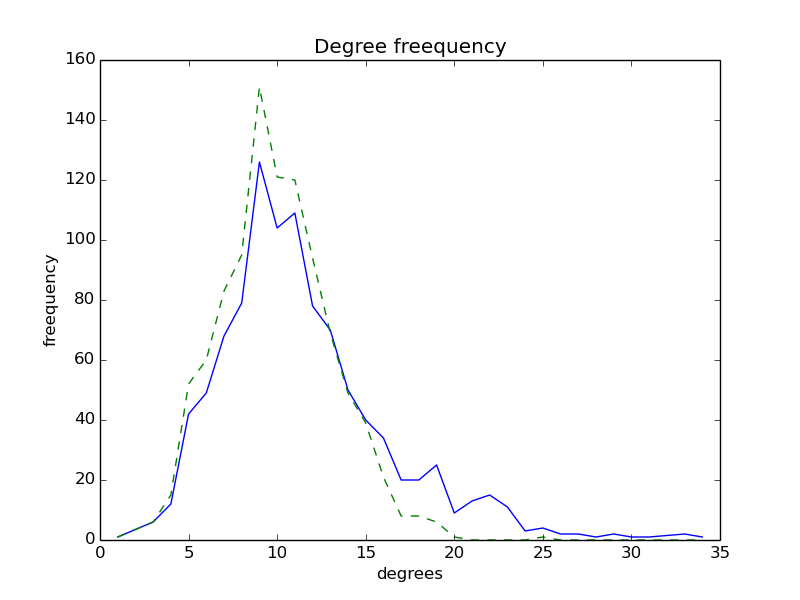
\includegraphics[scale=0.6]{images/n1000-e10000-sketches-810-820-823-827-830plot}
\caption[1000 nodes 10,000 edges with sketches of sizes 810, 820, 827, 830]{Degree distribution calculated on a graph with 1000 nodes 10,000 edges using set of sketches of sizes 810, 820, 827, 830}
\end{figure}

Then the metrics were calculated, which are Average Relative Error(ARE), Percentages of Effective Queries when $G_0$ is 0 (which is the number of queries giving the exact results), $G_0$ is 1, $G_0$ is 2 and $G_0$ is 3.

\paragraph{}

\begin{table}[H]
\centering
\begin{tabular}{|l|l|l|l|l|}
\hline
 ARE   & $G_0$=0 & $G_0$=1 & $G_0$=2 & $G_0$=3 \\ \hline
163.86 &   82.6  &   82.8  &   82.8  &   83.5  \\ \hline
\end{tabular}
\caption{Accuracy metrics for sketching}
\label{table:accuracy-metrics-for-sketching}
\end{table}


The experiment shows $82.6\%$ of the queries gave the exact same results and within $\pm3$ range approximation, there were $83.5\%$ queries giving correct results.

\section{Automatic sketch creation}
Here are the results of automatics sketch creation experiments. A series of experiments were carried out as this is where our extension to the TCM model comes in. 

\paragraph{}

First experiment used the node queries as in the previous experiments and calculated the degree distribution by asking every node in the graph for its degree. The experiment used ‘only one sketch gives correct value’ policy with 0 tolerance and 2 initial sketches of sizes 870, 910.

\paragraph{}

Here the automatic sketch creation was firstly run and then the number of sketches created and their sizes used was identified. Then the same experiment was done with the used number of sketches and with their respective sizes. 

\begin{figure}[H]
\centering
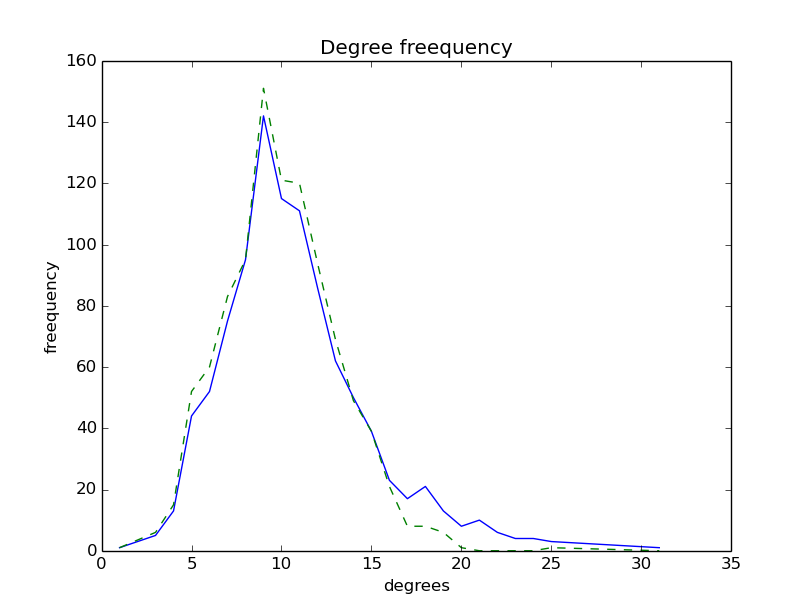
\includegraphics[scale=0.6]{images/ddas1}
\caption{Without automatic sketch creation, 1000 nodes, 10000 edges}
\end{figure}

\begin{figure}[H]
\centering
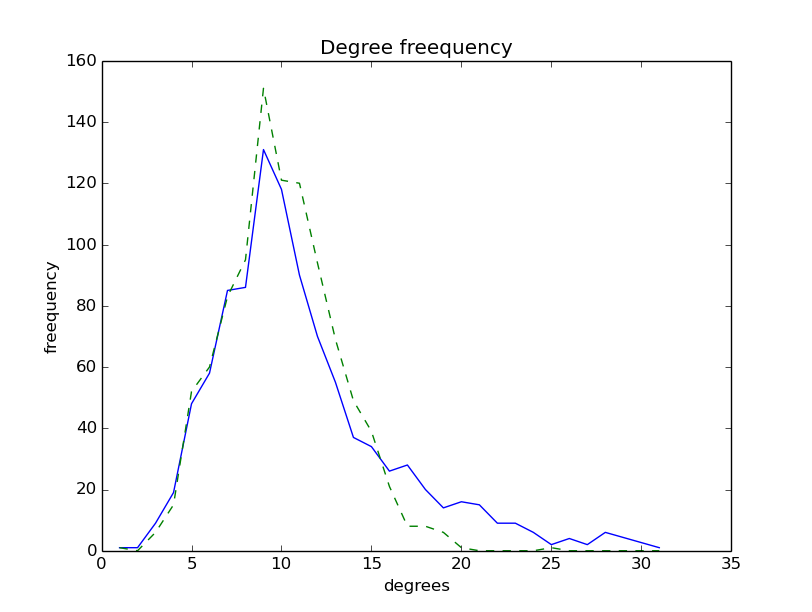
\includegraphics[scale=0.6]{images/ddas2}
\caption{With automatic sketch creation, 1000 nodes, 10000 edges}
\end{figure}

The results were satisfying when the two plots were visually compared and the next step was to do the same experiment with our defined accuracy metrics. 

\paragraph{}

In this experiment it was a graph with 1000 nodes and 10,000 edges was used with 'only two sketch gives correct value' policy with 0 tolerance and 2 initial sketches of sizes 810, 820. Automatic sketch creation mechanism had created altogether 5 sketches at the end with sizes 810, 820, 823, 827, 830.

\begin{figure}[H]
\centering
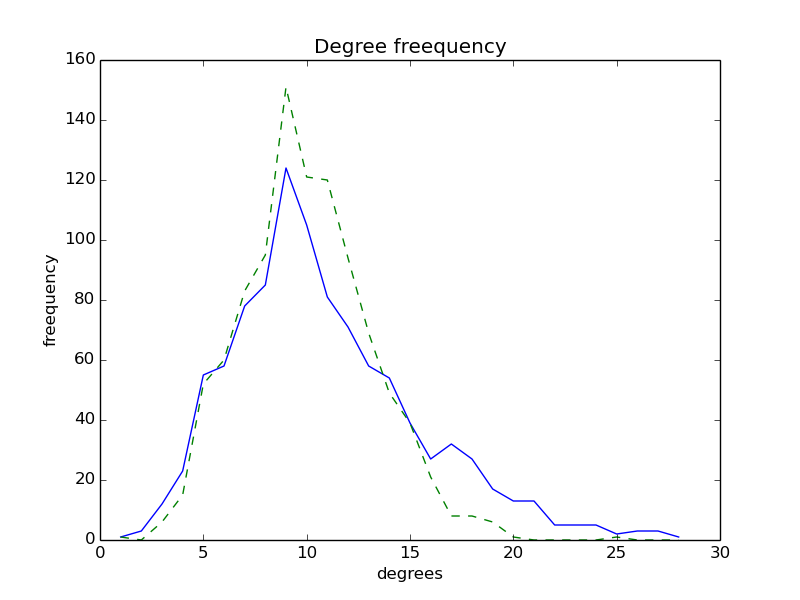
\includegraphics[scale=0.6]{images/AS-2init-2scale-0t-n1000-e10000-sketches-811-821-823-827-829plot}
\caption{1000 nodes and 10,000 edges was used with 'only two sketch gives correct value' policy}
\end{figure}

The accuracy metrics were as follows, 

\begin{table}[H]
\centering
\begin{tabular}{|l|l|l|l|l|l|}
\hline
 ARE   & $G_0$=0 & $G_0$=1 & $G_0$=2 &  $G_0$=3 & $G_0$=4 \\ \hline
200.80 &   58.5  &  65.8   &   73.3  &   79.8   &   81.8 \\ \hline
\end{tabular}
\caption{Accuracy metrics with automatic sketch creation}
\end{table}

Then the next experiment was done using the same number of sketches with same sizes, but without automatic creation, that is creating at the beginning. This way, we can benchmark the results of the automatic sketch creation with the results of the TCM with respect to accuracy measures. 

\begin{figure}[H]
\centering
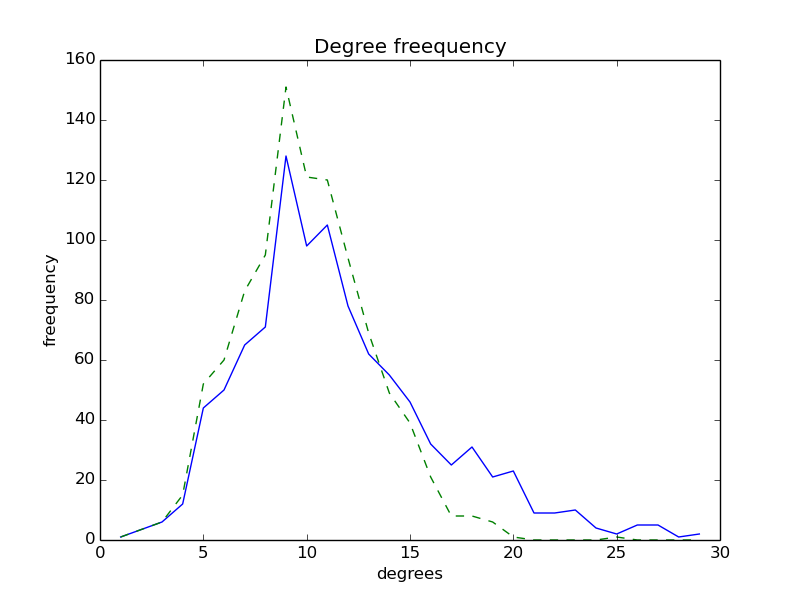
\includegraphics[scale=0.6]{images/MS-n1000-e10000-sketches-811-821-823-827-829plot}
\caption{1000 nodes, 10000 edges graph using sketches of sizes 810, 820, 823, 827, 830, without auto sketch creation}
\end{figure}

The accuracy metrics were as follows,

\begin{table}[H]
\centering
\begin{tabular}{|l|l|l|l|l|l|}
\hline
 ARE   & $G_0$=0 & $G_0$=1 & $G_0$=2 & $G_0$=3 & $G_0$=4\\ \hline
172.74 &   80.9  &   81.1  &   81.9  &   82.3  & 83.3   \\ \hline
\end{tabular}
\caption{Accuracy metrics for sketching without auto sketch creation}
\end{table}

The resulted Average Relative Error from the experiment which used automatic sketch creation, which is 200.80 was reasonable when compared to Average Relative Error  of the experiment which did not used the automatic sketch creation. 

\paragraph{}

How the effective queries are distributed over the error space was plotted and it gave the idea that many queries were in a favourable error range and very few queries were much deviated.

\begin{figure}[H]
\centering
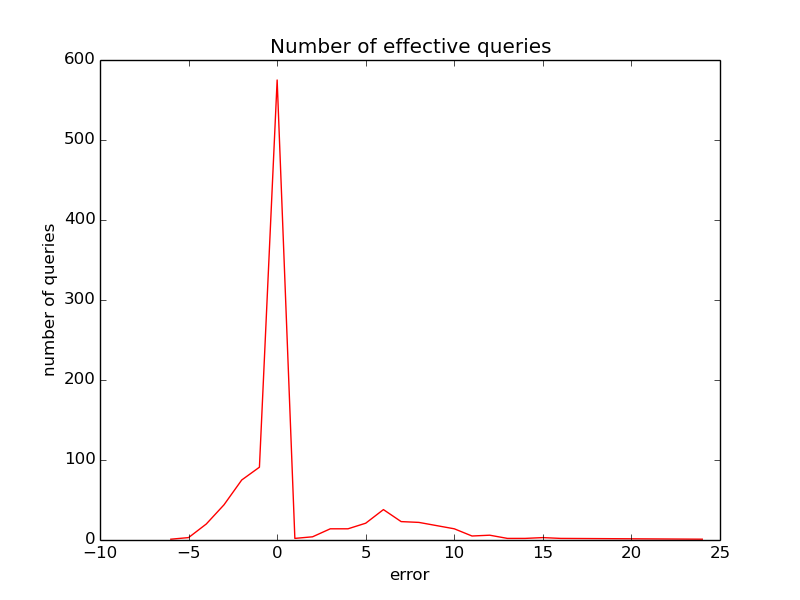
\includegraphics[scale=0.6]{images/deviation-plot-AS-2init-2scale-0t-n1000-e10000-sketches-811-821-823-827-829-839plot}
\caption{ Effective queries against the error space }
\end{figure}

\subsection{Effectiveness of the effective queries }

Then the next question was, if these effective queries are really effective? Let's say a degree of a node is 12 and the query gives it as 10, that is within an error of 2, which is acceptable. Let's take this as case 1. But if a degree of a node is 3 and the query gives it as 1, which is still within an error of 2, then this might not be acceptable for some needs. Let's take this as case 2.

\begin{figure}[H]
\centering
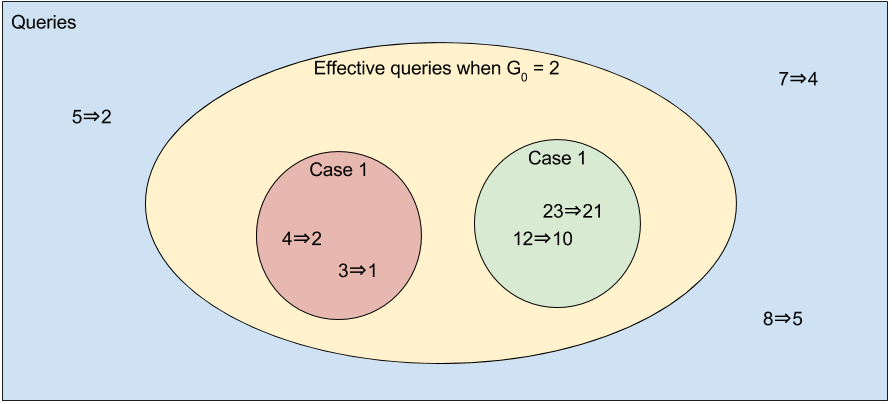
\includegraphics[scale=0.4]{images/Effective-queries-when-G-is-2}
\caption{Two cases of effective queries}
\end{figure}

\paragraph{}

Then this was investigated using a plot which evaluates the frequency of approximated queries over the degrees. In Figure \ref{fig:effective-queries-against-degree}, frequency of effective queries when $G_0$ is 1 are marked with the green line, frequency of effective queries when $G_0$ is 2 are marked with the orange line, frequency of effective queries when $G_0$ is 1 are marked with the purple line. 

\paragraph{}

This shows us the queries which were considered as effective are how effective. The queries which were considered effective when $G_0 = 1$ is starting from degree 3, which means, it is only the case where 3 is approximated to 2, is reasonable. Even the frequency of such approximated queries are low for smaller degrees. Majority of the queries which are considered as effective by approximation are on higher degrees, which is the case like 12 getting as 10.

\begin{figure}[H]
\centering
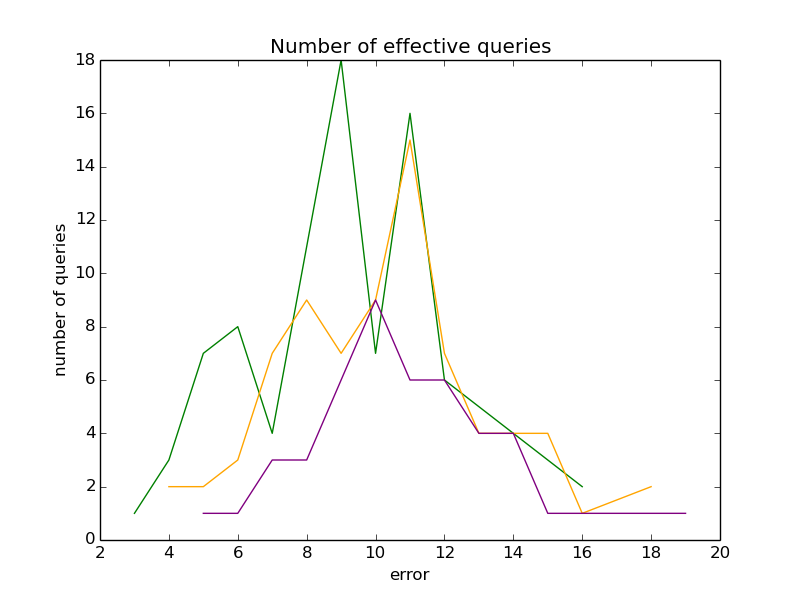
\includegraphics[scale=0.6]{images/deviation-plot-error-AS-2init-2scale-0t-n1000-e10000-sketches-811-821-823-827-829plot}
\label{fig:effective-queries-against-degree}
\caption{ Effective queries against the degrees }
\end{figure}

\subsection{Evaluating different creating policies}

Different automatic sketch creation policies were then evaluated using a 1000 nodes and  10000 edges graph on sketches of sizes 811, 821, 823, 827, 829 starting with 3 initial sketches.

\subsubsection{Only one sketch gives correct value}

\begin{table}[H]
\centering
\begin{tabular}{|l|l|l|l|}
\hline
 ARE   & $G_0$=0 & $G_0$=1 & $G_0$=2 \\ \hline
299.03 &   40.1  &   48.6  &   57.6  \\ \hline
\end{tabular}
\caption{Accuracy metrics for sketching using 'only one sketch gives correct value'}
\end{table}

\subsubsection{Only two sketch gives correct value}

\begin{table}[H]
\centering
\begin{tabular}{|l|l|l|l|}
\hline
 ARE   & $G_0$=0 & $G_0$=1 & $G_0$=2 \\ \hline
200.71 &   57.5  &   66.8  &   77.7  \\ \hline
\end{tabular}
\caption{Accuracy metrics for sketching using 'only two sketch gives correct value'}
\end{table}

\subsubsection{Only two sketch gives correct value, 1 tolerance}

\begin{table}[H]
\centering
\begin{tabular}{|l|l|l|l|}
\hline
 ARE   & $G_0$=0 & $G_0$=1 & $G_0$=2 \\ \hline
406.10 &   62.7  &   62.7  &     \\ \hline
\end{tabular}
\caption{Accuracy metrics for sketching using 'only two sketch gives correct value' and 1 tolerance}
\end{table}

As node queries were analysed to a greater extent, next move was to analyse how the system works for other types of queries. For the next analyses, edge queries were chosen.

\section{Experimenting with edge queries}

For the edge query experiment, the sketches were asked for the edge value giving two vertices. In the initial experiments, 10\% of the edges on the original graph were chosen randomly and then queried from the sketches. This way, when the graph has 1000 edges, 100 queries get performed in one experiment, and when graph has 10000 edges, 1000 queries get performed.

First experiment was done using 1000 nodes and 10000 edges and using sketches 145, 165, 170, 180. Number of Effective Queries were used as the accuracy measurements.

\begin{table}[H]
\centering
\begin{tabular}{|l|l|l|}
\hline
$G_0$=0 & $G_0$=1 & $G_0$=2 \\ \hline
97.74  &   99.99  &   100.0\\ \hline
\end{tabular}
\caption{Accuracy metrics for sketching with edge queries}
\end{table}

These results shows us the edge queries can produce quite accurate results using mush smaller sketches when compared to node queries. Then a series of experiment was performed with different edge sizes and the accuracy metrics were measured. Following are the some of the results.  

\begin{table}[H]
\centering
\begin{tabular}{|l|l|l|l|l|}
\hline
n    & e     & $G_0$=0 & $G_0$=1 & $G_0$=2 \\ \hline
1000 & 5000  & 99.44   & 100.00  & 100.00  \\ \hline
1000 & 10000 & 93.38   & 99.90   & 100.00  \\ \hline
1000 & 20000 & 66.25   & 95.57   & 99.77   \\ \hline
\end{tabular}
\caption{Accuracy metrics for sketching with edge queries on series of experiments}
\end{table}

\subsection{Confusion matrix for edge queries}

The next question was if the sketches were asked for edges which does not exist in the actual graph, then can the sketches identify this. An experiment was performed using a graph of 1000 nodes and 10,000. The the sketches was asked for 100 edges which did not existed in the original graph. 

\paragraph{}

\begin{table}[H]
\centering
\begin{tabular}{l|l|l|l}
\cline{2-3}
                                  & Sketch: Yes & Sketch: No &                            \\ \hline
\multicolumn{1}{|l|}{Actual: Yes} & 10000       & 0          & \multicolumn{1}{l|}{10000} \\ \hline
\multicolumn{1}{|l|}{Actual: No}  & 6          & 94        & \multicolumn{1}{l|}{100}  \\ \hline
                                  & 10006       & 94        &                            \\ \cline{2-3}
\end{tabular}
\caption{Confusion matrix for edge queries}
\end{table}

This shows the sketches could identify 94.0\% of the non-existing edges. Then the same experiment was  done with 1000 non-existing edges.

\paragraph{}

\begin{table}[H]
\centering
\begin{tabular}{l|l|l|l}
\cline{2-3}
                                  & Sketch: Yes & Sketch: No &                            \\ \hline
\multicolumn{1}{|l|}{Actual: Yes} & 10000       & 0          & \multicolumn{1}{l|}{10000} \\ \hline
\multicolumn{1}{|l|}{Actual: No}  & 64          & 946        & \multicolumn{1}{l|}{1000}  \\ \hline
                                  & 10064       & 946        &                            \\ \cline{2-3}
\end{tabular}
\caption{Confusion matrix for edge queries}
\end{table}

Again the sketches could identify 94.6\% of the non-existing edges accurately.


\subsection{Auto sketch creation with Edge Queries}

Now the automatic sketch creation was evaluated on edge queries with the accuracy metrics. The experiment used a graph of 1000 nodes and 10000 edges. Initial sketches were of sizes 73 and 79. 'only two sketch gives correct value' policy was used with 0 tolerance. The auto sketch creation mechanism had created 10 more sketches with sizes 83, 89, 111, 127, 137, 142, 157, 177, 191, 219.

\begin{table}[H]
\centering
\begin{tabular}{|l|l|l|}
\hline
$G_0$=0 & $G_0$=1 & $G_0$=2 \\ \hline
99.23  &   100.0  &   100.0\\ \hline
\end{tabular}
\caption{Accuracy metrics for sketching with edge queries using auto sketch creation}
\end{table}

Then the same experiment was carried out using the same number of sketches and same sketch sizes, but without automatic sketch creation, that is creating all the sketches at the beginning. The results were as follows.

\begin{table}[H]
\centering
\begin{tabular}{|l|l|l|}
\hline
$G_0$=0 & $G_0$=1 & $G_0$=2 \\ \hline
99.98  &   100.0  &   100.0\\ \hline
\end{tabular}
\caption{Accuracy metrics for sketching with edge queries without using auto sketch creation}
\end{table}

\paragraph{}

The experiments were done for large graphs and the accuracy were measured. Starting sketch sizes were chosen as 219 450. 

In this experiment, 'only two sketch gives correct value' policy was used with 2 tolerance, the auto sketch creation mechanism created 3 more sketches with sizes 555, 877, 999.  

\begin{table}[H]
\centering
\begin{tabular}{|l|l|l|l|l|}
\hline
n    & e     & $G_0$=0 & $G_0$=1 & $G_0$=2 \\ \hline
1000 & 10,000 & 99.90   & 99.99   & 100.00   \\ \hline
\end{tabular}
\caption{Accuracy metrics for sketching with edge queries on series of experiments}
\end{table}

In the next experiment, 'only two sketch gives correct value' policy was used with 2 tolerance, the auto sketch creation mechanism created 5 more sketches with sizes 555, 877, 999, 1005, 1560.  

\begin{table}[H]
\centering
\begin{tabular}{|l|l|l|l|l|}
\hline
n    & e     & $G_0$=0 & $G_0$=1 & $G_0$=2 \\ \hline
1000 & 100,000 & 99.83   & 99.91   & 100.00   \\ \hline
\end{tabular}
\caption{Accuracy metrics for sketching with edge queries on series of experiments}
\end{table}

The results shows us the automatic sketch creation also gives better results for edge queries.

\subsection{Dynamicness of the graph}

Other than the edge insertion, a graph stream might have edge deletions in some scenarios. How the accuracy of the model would hold when edge deletion happens was needed to be evaluated. An experiment was used to evaluate this, which deleted 1\% and 10\% of the edges in the graph and the other edges were queried. 


\begin{table}[H]
\centering
\begin{tabular}{|l|l|l|l|}
\hline
\%     & $G_0$=0 & $G_0$=1 & $G_0$=2 \\ \hline
1\% & 97.78   & 99.98   & 100.00   \\ \hline
10\% & 98.36   & 99.98   & 100.00   \\ \hline
\end{tabular}
\caption{Accuracy metrics with edge queries when the graph has edge deletions}
\end{table}

\section{Contribution of queries for accuracy in ASC}

Edge queries contributes in updating the new sketches, when performed. When an edge is retrieved, all the  sketches gives edge value as of their adjacency matrix, and new sketches which has not seen the edge gives a null, ∅. The returned edge values list could look like [ 9, 3, 2, 2, ∅ ] for instance. Here, when 2 gets selected as the correct value, that value can be set on the new sketch which gave a null, resulting an update in the new sketch. This way, when edge queries are performed, the sketches gets updated. 

\paragraph{}

However, the problem with node queries are, only one node is given. For example, when the degree of a node is asked, the cell values of corresponding row on the sketch's adjacency matrix are summed and returned. But when a new sketch which has not seen the node yet returns a null, the corresponding row on that sketch's adjacency matrix  can not be updated, because the other nodes which connects to the given node are not known. 

\paragraph{}

One problem with the previously done node query experiment was, this inability of node queries to contribute toward accuracy was not considered. Only the edge insertion has contributed to the accuracy in those experiments. Then a series of experiments was done performing a mix of edge queries and node queries and the accuracy metrics were measured.

\paragraph{}

Experiments used 1000 nodes and 10,000 graph and performed 1000 node queries. The first experiment performed 500 edge queries, that 5\% of the edges, the second used 10\% and the third used 20\%. 

\paragraph{}

\begin{table}[H]
\centering
\begin{tabular}{|l|l|l|l|l|}
\hline
\%    & ARE     & $G_0$=0 & $G_0$=1 & $G_0$=2 \\ \hline
0 & 0.200 &   58.5  &  65.8   &   73.3  \\ \hline
5\% & 0.194 & 60.8   & 71.8   & 76.1  \\ \hline
10\% & 0.187 & 66.2   & 77.4   & 80.1   \\ \hline
20\% & 0.173 & 80.2   & 80.9   & 80.9   \\ \hline
\end{tabular}
\caption{Accuracy metrics for automatic sketch creation  with edge queries and node queries on series of experiments}
\end{table}


The experiments showed a rise in accuracy of node queries when edge queries are performed with node queries. Only 58.5\% of the node queries gave exact accurate results when no edge queries are performed, and with 20\% of edge queries, the accuracy reached to 80.2\%.

\section{Evaluation on Natural graphs}

As being able to work with natural graphs is one objective of the research, final experiments were  about evaluating the model with natural graphs. 

\paragraph{}

First 2 experiments used 4 sketches with sizes 810, 820, 827, 830 and the accuracy metrics were calculated for node queries. The degree distribution was also plotted performing series of node queries the same way as previous node query experiments.

\paragraph{}

\begin{table}[H]
\centering
\begin{tabular}{|l|l|l|l|l|}
\hline
n    & e     & $G_0$=0 & $G_0$=1 & $G_0$=2 \\ \hline
1000 & 3166  & 89.8   & 95.9  & 97.9  \\ \hline
1500 & 7887 & 72.33   & 84.33   & 90.80  \\ \hline
\end{tabular}
\caption{Accuracy metrics for sketching with node queries on natural graphs}
\end{table}


\begin{figure}[H]
\centering
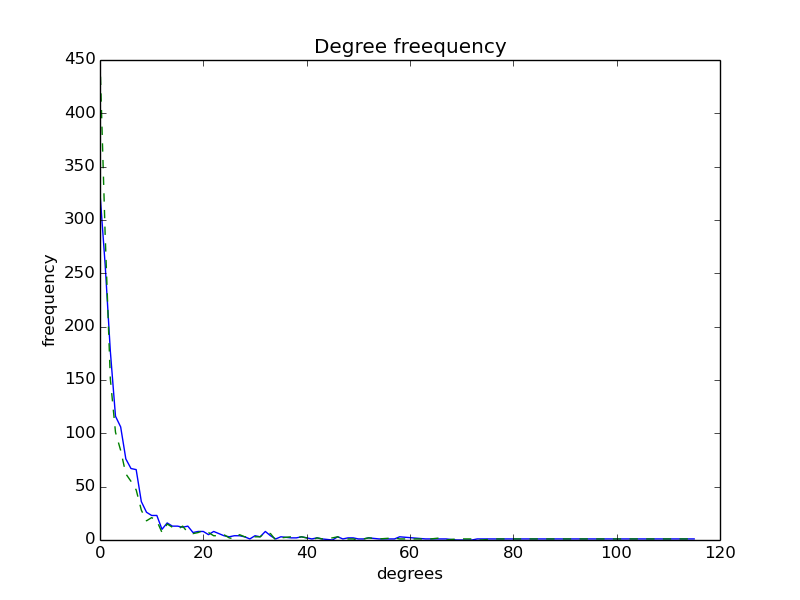
\includegraphics[scale=0.6]{images/GenForestFire-1000-035-035-n1500-e7887-sketches-810-820-827-830plot}
\end{figure}

Then the automatic sketch creation is evaluated using natural graph, starting with two initial sketches of sizes 810, 820. The automatic sketch creation mechanism then created 4 more sketches with sizes 827, 830, 870, 890.

\paragraph{}
 
\begin{table}[H]
\centering
\begin{tabular}{|l|l|l|l|l|}
\hline
n    & e     & $G_0$=0 & $G_0$=1 & $G_0$=2 \\ \hline
1000 & 4164  & 76.0   & 82.9  & 87.4  \\ \hline
\end{tabular}
\caption{Accuracy metrics for sketching with node queries on natural graphs when using automatic sketch creation}
\end{table}

These results shows the model is capable of working with natural graphs also, both when using automatic sketch creation and without using automatic sketch creation.

\section{Memory usage}
Table \ref{table:accuracy-metrics-for-sketching} shows the accuracy measures when using sketches on a 1000 nodes and 10000 edges graph. Within $\pm3$ range approximation, that is when $G_0$ is 3, there were $83.5\%$ queries giving correct results. When achieving this accuracy, the experiment used 4 sketches of sizes 810, 820, 827, 830. If we consider one cell of the adjacency matrix used one unit of memory, the the total memory used for all the 4 sketches would be, $810^2+820^2+827^2+830^2 = 2,701,329$. But if the number of nodes of the graph is knows before hand, one could create an adjacency matrix of size 1000 and that would take only $1000^2 = 1,000,000$ memory units. With sketches, the model has used approximately  2.7 times memory. 

\paragraph{}

However, as the number of nodes of the graph is not knows before hand, creating an adjacency list is not possible. If one created an adjacency matrix for N nodes, when the N+1 nodes arrives, the adjacency matrix can not accommodate the new node. But with sketching, number of nodes being larger than the sketch sizes is not a problem and the model can accommodate new nodes and still can produce an approximated result as shown in above experiments. 

\paragraph{}

One other thing is, all these sketches need not to be stored on one computation unit, but can be distributed on several units. Sketches are independent from each other, thus will not require communication between them as in graph partitioning where lot of inter partition communications happens. As the computations on sketches are independent, queries can be performed on sketches in parallel. On our sketching model, both node retrieval and edge retrieval can be done in constant time.  


\chapter{Conclusion and Future Work }

\section{Conclusion}

In our study we evaluated different techniques one could use to build a graph analysis model and looking at the strengths and weaknesses of these techniques we concluded on what techniques we should continue on and  how to solve the problems of the selected techniques. We moved from graph partitioning to one pass algorithms and then to graph summarising techniques. With graph summarising techniques we considered spanner, sparsifiers and sketchers. We continued with sketchers and identified TCM as a good sketching model. Then we implemented our model using TCM sketching and evaluated  the model with different scenarios and measures. We performed node queries and edge queries with different sketching setting and evaluated the accuracy using the Average Relative Error and Number of Effective Queries as accuracy  measurement. We also evaluated if the queries we consider as Effective are really effective. Then we evaluated the confusion matrix for the queries. The results were upto a reasonable satisfactory level. 

\paragraph{}

One problem with TCM sketching was, how it suggests to create the sketches is, to use the full available  memory in order to create sketches as large as possible. We questioned can't we extend the TCM to create the sketches dynamically as the graph grows? Two problems we had to solve for this was, when to create a new sketch and how. We introduced a heuristic based technique which looks at the sketch values and decide if a new sketch should be created and a techniques to create new sketches from existing sketches. Then we evaluated them the same way. Then we discussed and evaluated how the contribution of different queries towards the accuracy of the automatic sketch creation. The system was evaluated with natural graphs and dynamic graphs for accuracy and the accuracy of the automatic sketch creation mechanism was evaluated when working with natural graphs.

\paragraph{}

In both settings, that is, with and without automatic sketch creation, edge queries could produce better results than node queries, and node queries could produce better results when the sketch sizes are closer or larger to the number of nodes of the graph. Performing edge queries and node queries in a mix, as how it happens in real world scenarios, the accuracy of the node queries  increased in automatic sketch creation setting. Thus the model best fits for system where the number of edge are relatively high than nodes and edge queries and node queries happens in a mix. As the querying on sketches can be done in parallel, the model can respond to queries faster. As we have introduces a mechanism for creating sketches on the fly, we can create new sketches only when needed.

\section{Future Work}

The automatic sketch creation mechanism should be improved with identifying better heuristics for deciding when to created a new sketch. And also should identify if any better mechanisms for creating  and  updating  new sketches exists.  

\paragraph{}
This is an embarrassingly parallel query framework model, therefore the model should be evaluated on top of a parallel framework. And also, new metrics has to be defined for thorough evaluation

\newpage
\begin{appendices}


\chapter{Graph Analysis Frameworks}

\section{Pregel}
Pregel\cite{Pregel} is a graph framework for graph-parallel computations, where the computation is expressed as a sequence of steps, called ’supersteps’. In each step, a vertex receives a message from the previous step, changes its state and pass the message to the other vertices. Computation finishes when all the vertices are done and no more messages are passed. Since Pregel is a synchronous system, it updates parameters of each vertices in parallel using values from the previous step as input. One computation will take several rounds, that is several supersteps to complete. Partitioning of the graph is done by simply using a hash function on vertex ID as `partition = hash(ID) mod N` where the ID is the vertex ID and N is the number of partitions. 
 
\section{GraphLab}
GraphLab\cite{Graphlab} was introduced for dynamic and asynchronous graph-parallel computation. GraphLab consists of a Data Graph which holds the program state, an Update Function which is a stateless procedure that updates the Data Graph in small chunks called Scopes and a Sync Function which concurrently maintains global aggregates. Different hash functions are used to partition the graph. 


\section{Apache Giraph}
Giraph is an open source implementation of Google’s Pregel\cite{Pregel} graph processing architecture by Yahoo and Apache community. It is used at Facebook to analyse their huge one trillion edges graphs\cite{Facebook} formed by users and their interactions. Facebook has proposed several implementation-wise improvements in a paper\cite{Facebook}  published in 2015 such as how to keep vertices and edges in memory as pages instead objects to avoid Java Garbage Collector issues, how to run the processing in parallel with local multithreading to take advantage of additional CPU cores.
 
\section{Giraph++}
Giraph++\cite{GiraphPlusPlus} is an improved version of Apache Giraph which is an open source  implementations of Pregel which is graph centric rather vertex centric. Main difference between Pregel and Giraph++ is, in Giraph, the programmer can access the whole sub-graph in a partition, rather one vertex at a time.In Giraph++ each partition contains a set of vertices and all their outgoing edges. Each vertex is uniquely identified by an ID, and a partitioner decides which partition a vertex belongs to based on its ID. The partitioner is also used to route messages for a vertex correctly to its partition. The default partitioner is a hash function on the vertex ID.

\section{Apache Spark’s GraphX}
Apache Spark is a very popular open source cluster computing framework for large-scale data processing. However, Apache Spark is micro-batching based and not truly real-time. 

\paragraph{}

Apache Spark’s graph abstraction package GraphX has gained lot of attention in the developer community for their graph based computational needs. GraphX also uses Pregel, but its own optimized variant of Pregel, in its underneath implementation.

\paragraph{}

GraphX is a thin layer on top of Spark for graph processing. GraphX simplify graph computation to a specific join-map-group-by dataflow pattern. Vertex-cut partitioning is used to encode graphs as horizontally partitioned collections. 

\section{Apache Flink’s Gelly}
Apache Flink is a relatively new data stream processing framework like Apache Spark, but has gained a lot of attention recently in the developer and research communities. Like Apache Spark, Flink is a streaming framework where we can plug different data streams and run different types of data analysis jobs on it. 

\paragraph{}

Apache Flink have a graph framework called Gelly, which run on top of Flink, like Apache Spark has GraphX. However, Gelly is only for static graph processing. 

\paragraph{}

However, there is a research on how to extend to Gelly to support streaming. They have used Flink’s shared states to continue the graph across iterations of the stream. We will be discussing that under One Pass Algorithms. 

\section{Titan}
Titan\cite{Titan} is a distributed graph database engine of OLTP type, build on top of Cassandra as the underlying data storage, but which now supports other data storage systems like HBase and BerkeleyDB. Titan natively supports the Gremlin Server component of the Tinkerpop stack. Titan’s storage model is an adjacency list in a column family where row key is vertex id. Titan maintains indexes in a separate column family and one nice feature of Titan is its ability to accommodate third party tools like Elasticsearch, Lucene, etc for indexing. 

\chapter{Graph Partitioning algorithms}

\section{PowerGraph}
PowerGraph\cite{PowerGraph} accommodates a sequential greedy heuristic which places the next edge on the machine that minimizes the conditional expected replication factor. The steps are simple.  If A(u) and A(v) are adjacencies of u and v respectively,

Case 1: If A(u) and A(v) intersect, then the edge should be assigned to a machine in the intersection.

Case 2: If A(u) and A(v) are not empty and do not intersect, then the edge should be assigned to one of the machines from the vertex with the most unassigned edges.

Case 3: If only one of the two vertices has been assigned, then choose a machine from the assigned vertex.

Case 4: If neither vertex has been assigned, then assign the edge to the least loaded machine.

\section{Linear Deterministic Greedy}
This consider two important factors when  assigning a vertex to a partition.  They are, how related a vertex to other vertices in a given partition and the capacity remaining in the partition. P\textsuperscript{t}\textsubscript{i}  denotes the ith partition in the given time t, C\textsubscript{i} denotes the capacity of the i\textsuperscript{th} partition. N(u) means the neighbors of vertex u. 

\begin{figure}[H]
\centering
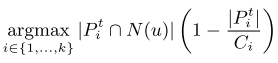
\includegraphics[scale=0.5]{images/image07}
\end{figure}

\section{X-stream}
X-stream\cite{XStream}is proposing streaming partitioning for bounded graphs, that is the vertices and edges remains fixed during the entire computation and the number of partitions stays fixed throughout the computation. The design is motivated by the fact that sequential bandwidth for all storage media (main memory, SSD, etc) is substantially larger than random access bandwidth and a large number of graph algorithms can be expressed using the edge-centric scatter-gather model. 

\paragraph{}

During initialization, the vertex set of the entire graph is partitioned into vertex sets for the different partitions, and the edge list of each partition is computed. 

\section{S-PowerGraph}
S-PowerGraph\cite{S-PowerGraph} discuss several methods as ’Degree’, a greedy procedure which makes use of the in-degree distribution and ’DegreeIO’ which tries to meet the challenge that both indegree and outdegree of natural graphs are skewed. 

\paragraph{}

S-PowerGraph firstly suggests the Grid-based Constrained Random Vertex-cut algorithm of GraphBuilder[?] could be altered for streaming graph partitioning. In this method, a vertex is mapped into a shard which accommodates a constrained set of partitions. Then, the partition a vertex to be assigned will be chosen from the constrained set randomly. The edge e is assigned to P\textsubscript{idx} where idx is decided by idx = GridHash(e), the hash function implemented in GraphBuilder. 

\paragraph{}

Then the S-PowerGraph discuss about an enhanced version of the greedy algorithm proposed in PowerGraph\cite{PowerGraph}. As the greedy algorithm in PowerGraph could lead to some unbalanced partitions in some cases, they introduce Balance(PowerGraph) where Balance() is a constraint to avoid the imbalance.

\paragraph{}

\section{Linear Embedding}
”Distributed Balanced Partitioning via Linear Embedding”\cite{Linear Embedding} discusses a method researchers at Google have tried and tested with Google services. ”Linear Embedding” is a balanced partitioning problem where the goal is to partition the vertices of a given graph into k parts so as to minimize the total cut size. Linear Embedding method first embeds nodes of the graph onto a line, then attempt to improve the ordering mainly by swapping vertices in a semi local manner and finally accommodate a post-processing method to improve the cut-size.

\paragraph{} 

They discuss several different methods for each different step and compare the outcome performances for each combination. For embedding nodes onto a line, they accommodate random mapping, Hilbert curve mapping when geographic/geometric information is available, and Affinity-based mapping which takes into account the affinity of vertices by grouping vertices that are closely connected, hence building a tree of these connections. Once the linear embedding is done, the next step is to improve ordering using semi local moves. One method is using Minimum Linear Arrangement (MinLA)\cite{MinLA} and the other is Rank Swap which depends on the pre chosen cut boundaries, the number of final partitions k.




\end{appendices}


\begin{thebibliography}{1}

  \bibitem{PageRank} Page, L., Brin, S., Motwani, R.,  Winograd, T. (1998). The PageRank Citation Ranking: Bringing Order to the Web. World Wide Web Internet And Web Information Systems, 54(1999-66), 1–17. http://doi.org/10.1.1.31.1768
  \bibitem{Horawalavithana} Horawalavithana, Y. S. (2015). Cloud based publish / subscribe model for Top-k matching over continuous data streams. Undergraduate Thesis, University of Colombo
  \bibitem{TwitterStats} "Twitter: Number Of Active Users 2010-2016 | Statista". Statista. N.p., 2016. Web. 30 Dec. 2016.
  \bibitem{Facebook} Ching, A., Edunov, S., Kabiljo, M., Logothetis, D.,  Muthukrishnan, S. (2015). One Trillion Edges : Graph Processing at Facebook-Scale. Vldb, 8(12), 1804–1815. http://doi.org/10.14778/2824032.2824077
  \bibitem{WebGraphs} S. Raghavan and H. Garcia-Molina. Representing web graphs. In ICDE, pages 405–416, Atlanta, GA, USA, 2003.
  \bibitem{PowerGraph} Gonzalez, Joseph E et al. "Powergraph: Distributed graph-parallel computation on natural graphs." Presented as part of the 10th USENIX Symposium on Operating Systems Design and Implementation (OSDI 12) 2012: 17-30.

  \bibitem{Pregel}  Malewicz, Grzegorz et al. "Pregel: a system for large-scale graph processing." Proceedings of the 2010 ACM SIGMOD International Conference on Management of data 6 Jun. 2010: 135-146.

  \bibitem{Graphlab} Low, Yucheng et al. "Graphlab: A new framework for parallel machine learning." arXiv preprint arXiv:1408.2041 (2014).
  
  \bibitem{DistributedGraphLab} Low, Y., Gonzalez, J., Kyrola, A., Bickson, D.,  Guestrin, C. (2011). Distributed GraphLab: A Distributed Framework for Machine Learning in the Cloud, 716–727. http://doi.org/10.14778/2212351.2212354
  
  \bibitem{S-PowerGraph} Xie, Cong, Wu-Jun Li, and Zhihua Zhang. "S-PowerGraph: Streaming Graph Partitioning for Natural Graphs by Vertex-Cut." arXiv preprint arXiv:1511.02586 (2015).
  
  \bibitem{Graphbuilder} Jain, Nilesh, Guangdeng Liao, and Theodore L Willke. "Graphbuilder: scalable graph etl framework." First International Workshop on Graph Data Management Experiences and Systems 23 Jun. 2013: 4.
  \bibitem{Linear Embedding} Aydin, Kevin, MohammadHossein Bateni, and Vahab Mirrokni. "Distributed Balanced Partitioning via Linear Embedding." arXiv preprint arXiv:1512.02727 (2015).
  \bibitem{MinLA} Goldschmidt, Olivier, and Dorit S Hochbaum. "Polynomial algorithm for the k-cut problem." (1988): 444-451.
  \bibitem{Titan} "big graph data with cassandra - DataStax." 2012. 25 May. 2016 http://www.datastax.com/wp-content/uploads/2012/08/C2012-Titan-MatthiasBroecheler.pdf
  \bibitem{GiraphPlusPlus} Tian, Y., Balmin, A., and Corsten, S. (2013). From "think like a vertex" to "think like a graph." Proceedings of the VLDB Endowment, 7, 193–204. http://doi.org/10.14778/2732232.2732238
  \bibitem{GraphX} Xin, R. S., Gonzalez, J. E., Franklin, M. J., Stoica, I.,  AMPLab, E. (2013). GraphX: A Resilient Distributed Graph System on Spark. First International Workshop on Graph Data Management Experiences and Systems. http://doi.org/10.1145/2484425.2484427
  \bibitem{Fennel} Tsourakakis, C., Gkantsidis, C., Radunovic, B.,  Vojnovic, M. (2014). Fennel: Streaming graph partitioning for massive scale graphs. Proceedings of the 7th ACM International Conference on Web Search and Data Mining, 333–342. http://doi.org/10.1145/2556195.2556213
  \bibitem{X-stream} Roy, A., Mihailovic, I.,  Zwaenepoel, W. (2013). X-stream: edge-centric graph processing using streaming partitions. The Twenty-Fourth ACM Symposium on Operating Systems Principles, 472 – 488. http://doi.org/10.1145/2517349.2522740
  \bibitem{GraphSketches}Kook Jin Ahn, Sudipto Guha, and Andrew McGregor. 2012. Graph sketches: sparsification, spanners, and subgraphs. In Proceedings of the 31st ACM SIGMOD-SIGACT-SIGAI symposium on Principles of Database Systems (PODS '12), Markus Krötzsch (Ed.). ACM, New York, NY, USA, 5-14. DOI=http://dx.doi.org/10.1145/2213556.2213560
  \bibitem{Kalavri} Kalavri, V. (n.d.). Batch and Stream Graph Processing with Apache Flink.
  \bibitem{CountMin} Cormode, G., and Muthukrishnan, S. (2005). An improved data stream summary: The count-min sketch and its applications. Journal of Algorithms, 55(1), 58–75. http://doi.org/10.1016/j.jalgor.2003.12.001
  \bibitem{gSketch} Zhao, P., Aggarwal, C. C., Watson, I. B. M. T. J., and Ctr, R. (2011). gSketch : On Query Estimation in Graph Streams. Vldb, 5(3), 193–204. http://doi.org/10.14778/2078331.2078335
  \bibitem{TCM} Tang, N., and Chen, Q. (2016). Graph Stream Summarization From Big Bang to Big Crunch. [SIGMOD]
  \bibitem{GMatrix} Khan, A., and Aggarwal, C. (2016). Query-Friendly Compression of Graph Streams.
  \bibitem{powerLaw1}Mitzenmacher, M. (2004). A Brief History of Generative Models for Power Law and Lognormal Distributions. Internet Mathematics, 1(2), 226–251. http://doi.org/10.1080/15427951.2004.10129088
  \bibitem{powerLaw2}Xie, C., Yan, L., Li, W.-J., and Zhang, Z. (2014). Distributed Power-law Graph Computing: Theoretical and Empirical Analysis. Nips, 1673--1681. Retrieved from http://papers.nips.cc/paper/5396-distributed-power-law-graph-computing-theoretical-and-empirical-analysis.pdf
  \bibitem{frequency counts}G. S. Manku and R. Motwani. Approximate frequency counts over data streams. In VLDB, pages 346–357, 2002
  \bibitem{Vitria} Vitria. http://www.vitria.com/solutions/streaming- big-data-analytics/benefits/
  \bibitem{sparse spanners}M. Elkin. Streaming and fully dynamic centralized algorithms for constructing and maintaining sparse spanners. ACM Transactions on Algorithms,7(2):20, 2011.
  \bibitem{Spectral sparsification} J. A. Kelner and A. Levin. Spectral sparsification in the semi-streaming setting. Theory Comput. Syst., 53(2):243–262, 2013.
  \bibitem{Graph stream algorithms survey}A. McGregor. Graph stream algorithms: a survey. SIGMOD Record,43(1):9–20, 2014.
  \bibitem{HeavyHitters}G. Cormode and S. Muthukrishnan. Space efficient mining of multigraph streams. In PODS, pages 271–282, 2005.
  \bibitem{Graph sketches}Ahn, K. J., Guha, S.,  McGregor, A. (2012). Graph sketches: sparsification, spanners, and subgraphs. Proceedings of the 31st Symposium on Principles of Database Systems, 2012(Pods), 5–14.
  \bibitem{Streaming Balanced Graph Partitioning Algorithms2}Stanton, I. (2014). Streaming Balanced Graph Partitioning Algorithms for Random Graphs. Soda, 1287–1301. http://doi.org/10.1137/1.9781611973402.95
  \bibitem{Streaming Balanced Graph Partitioning Algorithms1}Kliot, G.,  Stanton, I. (2012). Streaming Graph Partitioning for Large Distributed Graphs. Acm Kdd, 1222–1230. http://doi.org/10.1145/2339530.2339722
  
  
  
\end{thebibliography}
\end{document}